\documentclass[a4paper,10pt,twoside]{report}

% Packages for enhancing LaTeX capabilities
\usepackage[a4paper, inner=4cm, outer=3cm, top=2.5cm, bottom=2.5cm]{geometry}
\usepackage{fontspec}
\usepackage{setspace}
\usepackage{fancyhdr}
\usepackage{graphicx}
\usepackage[backend=biber,style=apa]{biblatex}
\usepackage{csquotes}
\usepackage[ngerman]{babel}
\usepackage{float}
\usepackage{amsmath}
\usepackage{fancyhdr}
\usepackage{longtable}
\usepackage{array}
\usepackage{rotating}

\raggedbottom


\setmainfont{Arial}
\setlength{\baselineskip}{1.2\baselineskip}
\pagenumbering{roman}
\addbibresource{../../Ressourcen/Bibliographie/ba_literatur.bib}


\begin{document}

% Titlepage
\begin{titlepage}
  \hspace*{\fill}
  
\includegraphics[width=0.4\textwidth,keepaspectratio]{../../Ressourcen/Bilder/FHE-AI_Logo.png}

  \centering
  \vspace*{1cm}

  \vspace{0.5cm}

  {\Huge\textbf{Bachelorarbeit in der Angewandten Informatik}}
  \\
  Registriernummer: AI-2024-BA-030

  \vspace{1.5cm}

  {\large\textbf{Konzeption und Entwicklung einer datenbankseitigen Abbildung von frei definierbaren Bilanzräumen
      im Zusammenhang mit dem Energiemanagementsystem EMS-EDM PROPHET® nach ISO 50001.}}

  \vspace{1.5cm}

  {\Large\textbf{Fabian Heinlein}}
  \\ in Kooperation mit dem Fraunhofer Institut Angewandte Systemtechnik (IOSB-AST)

  \vspace{1cm}

  \Large Abgabedatum: 28.02.2024

  \vspace{1cm}

  Prof. Dr. Marcel Spehr \\
  Sven Möller

  \vfill

\end{titlepage}

\setcounter{page}{1}



\chapter*{Kurzfassung}
\addcontentsline{toc}{chapter}{Kurzfassung}
\chapter*{Abstract}
\addcontentsline{toc}{chapter}{Abstract}
\chapter*{Vorwort}
\addcontentsline{toc}{chapter}{Vorwort}
\tableofcontents

%%%%%%%%%%%%%%%%%%%%%%%%%% Einleitung %%%%%%%%%%%%%%%%%%%%%%%%%%
\chapter{Einleitung}
\pagenumbering{arabic}
\setcounter{page}{1}

\section{Hintergrund und Motivation}
Angesichts wachsender Umweltbelastungen und der Notwendigkeit nachhaltiger Praktiken spielt das Energiemanagement eine immer bedeutendere Rolle.
Diese Arbeit untersucht die Entwicklung einer datenbankseitigen Lösung zur Abbildung frei definierbarer Bilanzräume im Energiemanagementsystem
EMS-EDM PROPHET® nach DIN EN ISO 50001:2018-12.
Sie wird durch das Potenzial, bei der Verbesserung der energiebezogenen Leistung und Energieeffizienz von Organisationen im tertiären Wirtschaftssektor 
durch die Erfüllung ausgewählter Kriterien der DIN EN ISO 50001:2018-12 zu unterstützen, motiviert. 
Bilanzräume stellen das zentrale Konzept der Arbeit dar und werden im Rahmen dieser als Einheiten betrachtet, die zur digitalen Abbildung 
von Organisationsstrukturen im Energiemanagement und als administrative Grenze zur Bilanzierungsrechnung dienen.
Die Adressierung der Arbeit auf die freie definierbare Gestaltung der Bilanzräume soll eine Möglichkeit bieten, der Diversität von Organisationen innerhalb des 
tertiären Wirtschaftssektors gerecht zu werden
und einen Einsatz der Forschungsergebnisse in solchen Organisationen mit dem EDM-EMS-Prophet® ermöglichen.
Die Untersuchung soll zur Weiterentwicklung nachhaltiger Energiemanagementpraktiken beitragen und Einblicke in die Integration
technischer Lösungen in bestehende Systeme bieten.

Ein wesentlicher Fokus dieser Arbeit liegt auf der DIN EN ISO 50001:2018-12, einer Norm der Internationalen Organisation für Normung (ISO),
die Anforderungen an Energiemanagementsysteme festlegt. Diese Norm ist universell einsetzbar, unabhängig von Größe, Art oder Standort der Organisation (\cite[S. 10]{DIN50001.2018}),
und dient der fortlaufenden Verbesserung der energiebezogenen Leistung. (\cite[S. 7]{DIN50001.2018}).
Um die Anforderungen der DIN EN ISO 50001:2018-12 zu erfüllen, müssen Organisationen den kontinuierlichen Fortschritt ihrer energiebezogenen Leistung nachweisen, wobei
die Norm keine spezifischen Zielniveaus vorgibt. (\cite[S. 10]{DIN50001.2018}).

Die Umsetzung der DIN EN ISO 50001:2018-12 in Organisationen bringt sowohl operationale als auch organisatorische Herausforderungen mit sich [S. 11](\cite{Marimon.2017}).
Dennoch lag im Jahr 2023 in 24.924 Organisationen weltweit ein Zertifikat nach DIN EN ISO 50001:2018-12 vor (\cite{InternationalOrganizationforStandardization.2023}).
Dies ist bemerkenswert, da die Erfüllung der Normanforderungen voraussichtlich etwa 60 \% des globalen Energieverbrauchs beeinflussen
kann (\cite{InternationalOrganizationforStandardization.2011}, zitiert nach \cite[S. 1]{Marimon.2017}). Darüber hinaus entstehen für Organisationen durch
die Einführung der Norm signifikante Vorteile.

Zum einen können nach Aussagen der DIN EN ISO 50001:2018-12 (2018, S. 9) ökonomische Vorteile wie Energieeinsparungen erzielt werden, wodurch Organisationen einen Wettbewerbsvorteil
aufgrund sinkender Energiekosten erlangen können. Zum anderen ergeben sich operationale Vorteile wie eine gesteigerte Produktivität, verbesserte Qualität
und ein strukturierter Ansatz zur Prozessoptimierung (\cite{Marimon.2017}). Des Weiteren kann die Umsetzung der DIN EN ISO 50001:2018-12 dazu beitragen, die allgemeinen
Klimaschutzziele zu erreichen (\cite{DIN50001.2018}). Dies unterstreicht die gesellschaftliche Bedeutung der Norm, insbesondere angesichts der Herausforderungen
des Klimawandels.

Die Umsetzung der DIN EN ISO 50001:2018-12 basiert auf dem PDCA-Zyklus (Plan, Do, Check, Act), der Organisationen einen strukturierten Rahmen für die fortlaufende
Verbesserung der energiebezogenen Leistung bieten soll (\cite[S. 7f.]{DIN50001.2018}).
Während die Norm in erster Linie Anforderungen auf Managementebene formuliert, verweist sie auch auf technische Normen wie die E DIN ISO 50006:2024-07, die unter anderem
spezifische Anforderungen an Energieleistungskennzahlen und energetische Ausgangsbasen definiert (\cite{DIN50006.2024,DIN50001.2018}).


\section{Problemstellung}
\subsection{Problembeschreibung}
\textbf{Forschungsfrage:} "Welche strukturellen Erweiterungen und Anpassungen müssen auf Datenbankebene in EMS-EDM PROPHET® konzipiert und implementiert 
werden, um eine frei definierbare Abbildung von Bilanzräumen zu ermöglichen, die Organisationen bei der Erfüllung der ISO 50001 unterstützt?"

Die breite Anwendbarkeit der in der DIN EN ISO 50001:2018-12 gestellten Anforderungen auf Organisationen führt zu Anforderungen an die Abbildbarkeit von 
frei definierbaren energiebezogenen Organisationsstrukturen im Energiemanagementsystem.

Ein Teilaspekt zur Umsetzung der DIN EN ISO 50001:2018-12 im Rahmen der Energiebilanzierung ist die Abbildung von energiebezogenen Bereichen in 
Organisationen im Energiemanagementsystem und soll im Rahmen dieser Arbeit betrachtet werden.

Die aktuelle Datenbankstruktur von EMS-EDM Prophet® steht vor dem Problem, frei definierbare Bilanzräume abzubilden.
Um dieses Problem zu lösen, sind strukturelle Änderungen und Erweiterungen der Datenbank notwendig.
Somit besteht das zentrale Problem dieser Arbeit darin, ein System zur Abbildung frei definierbarer Bilanzräume auf Datenbankebene unter Berücksichtigung 
der von der DIN EN ISO 50001:2018-12 gestellten Anforderungen an Bilanzräume und damit verbundene Themenkomplexe in EMS-EDM Prophet® zu konzipieren und 
zu implementieren.

Die Problemlösung umfasst alle Aspekte, die auf Grundlage der Vorgaben der Norm sowie praktischer Gegebenheiten konzipiert und auf Datenbankebene 
umgesetzt werden müssen, um EMS-EDM PROPHET® so zu erweitern, dass das System in der Lage ist, Organisationen bei der Erfüllung der ISO 50001 zu 
unterstützen. Dies gilt insbesondere für Anforderungen, die durch die Abbildung von Bilanzräumen adressiert werden können.

Aufgrund der Anwendbarkeit der DIN EN ISO 50001:2018-12 auf alle Organisationen ist die freie Definierbarkeit der Bilanzräume ein Qualitätskriterium des zu 
entwerfenden Systems und spielt bei der Beantwortung der Forschungsfrage eine zentrale Rolle.
Die breite Anwendbarkeit der Norm impliziert außerdem die Notwendigkeit, praktische Herausforderungen beim Einsatz der Lösung zu berücksichtigen und 
Anwendungsgebiete des entworfenen Konzepts zu betrachten, um der praktischen Relevanz dieser Arbeit gerecht zu werden.

\subsection{Praktische Relevanz des Problemraums} 
Das beschriebene Problem weist eine praktische Relevanz auf, da es die Herausforderungen der DIN EN ISO 50001:2018-12
im Energiemanagement von Organisationen adressiert.
Die bestehenden Anforderungen der DIN EN ISO 50001:2018-12 und der aktuelle Zustand von EMS-EDM Prophet® stellen praxisnahe Qualitätskriterien an die Abbildung von Bilanzräumen.
Eine Herausforderungen besteht darin, ein Datenbankmodell zu entwickeln, das diese Anforderungen erfüllt und gleichzeitig praxisnah und umsetzbar ist.
Die Berücksichtigung von aus der Praxis abgeleiteten Anforderungen ist dabei unerlässlich.
Dies verdeutlicht die Notwendigkeit einer Methodik, die sowohl theoretische als auch praktische Aspekte integriert.
Die Integration der Lösung in EMS-EDM Prophet® stellt sicher, dass sie in bestehenden Organisationen nutzbar ist und deren Energiemanagement unterstützt.

\subsection{Wissenschaftliche Relevanz des Problemraums} 
Die Problemstellung weist eine wissenschaftliche Relevanz auf, da im Zuge der Erarbeitung einer Lösung Methoden des Datenmanagements im Kontext der 
Modellierung von Energiebilanzräumen angewandt werden.
Dabei werden die in EMS-EDM Prophet® bestehenden Methoden um neue Ansätze zur Modellierung von Bilanzräumen erweitert.
Diese Erweiterungen tragen zur wissenschaftlichen Diskussion über Datenmanagementstrategien im Energiemanagement bei und bieten neue Perspektiven für die 
Integration von Bilanzräumen in datenbankbasierte Systeme.
Darüber hinaus fördert die Arbeit den interdisziplinären Austausch zwischen den Bereichen Energiemanagement und Datenbankmodellierung, indem sie 
theoretische Konzepte mit praktischen Anwendungen verknüpft.
Die entwickelten methodischen Ansätze und Modelle können als Grundlage für zukünftige wissenschaftliche Untersuchungen dienen und die Weiterentwicklung 
von Energiemanagementsystemen unterstützen.


\section{Ziel der Arbeit}

Das Ziel dieser Arbeit ist die Konzeption, Implementation und Evaluation eines Prototyps, der durch strukturelle Anpassungen und 
Erweiterungen des EMS-EDM Prophet® die Abbildung frei definierbarer Bilanzräume ermöglicht. Der Prototyp soll einen Mehrwert zur 
Erfüllung der Anforderungen der DIN EN ISO 50001:2018-12 bieten und in Organisationen des tertiären Wirtschaftssektors, die EMS-EDM Prophet® nutzen, 
anwendbar sein. Die Erarbeitung des Prototyps soll auf den theoretischen Grundlagen des Daten- und Energiemanagements basieren und bewährte Ansätze 
aus den Bereichen verwenden. Außerdem soll der Prototyp praktische Herausforderungen in den potentiellen Anwendungsgebieten berücksichtigen und 
allgemeine Anforderungen an Organisationen zu dessen Umsetzung formulieren.


Zur Evaluation des Prototyps soll die Bilanzraumstruktur der Organisation: Fraunhofer IOSB-AST in Ilmenau im entworfenen Prototyp abgebildet werden.
Der angewendete Prototyp soll im Bezug auf die unterstützung bei der Erfüllung der DIN EN ISO 50001:2018-12 Anforderungen auf qualitative und quantitative 
Qualitätskriterien evaluiert werden.
Außerdem soll die freie Definierbarkeit und die praktische Anwendbarkeit des Prototyps evaluiert werden.



\section{Aufbau der Arbeit}
Diese Arbeit ist so konzipiert, dass Sie die theoretischen Grundlagen des Problemraums erfasst und Nutzen sowie Herausforderungen im Anwendungsgebiet: 
EMS nach DIN EN ISO 50001:2018-12 erarbeitet. 
Basierend auf den theoretischen Grundlagen im Anwendungsbereich und den bestehenden Methoden und Ansätzen des Datenmanagements 
in EMS-EDM Prophet® wird eine Lösung der Forschungsfrage auf Datenbankebene des Energiemanagementsystems konzipiert, 
implementiert und evaluiert.
Der Aufbau der Arbeit umfasst drei Hauptabschnitte: die theoretischen Grundlagen und der Stand der Wissenschaft, die Konzeption und Implementation, und die 
Evaluation.

\begin{enumerate}
    \item \textbf{Theoretische Grundlagen und Stand der Wissenschaft}
    
    Die praxisnahe Problemstellung erfordert eine anwendungsorientierte Forschung unter Berücksichtigung der Interdisziplinarität. 
    Im theoretischen Teil der Arbeit werden zwei Themenbereiche betrachtet: Grundlagen der Energiebilanzierung unter Nutzung von Bilanzräumen und  
    Energiemanagementsysteme nach DIN EN ISO 50001:2018-12. In beiden Tehemenbereichen findet die erarbeitung der Grundlagen unter beachtung des Anwendungsgebiets: 
    Organisation im tertiären Wirtschaftssektor statt. 
    
    Für die Erarbeitung der theoretischen Grundlagen des Energiemanagements werden im ersten Hauptabschnitt der Arbeit die DIN EN ISO 50001:2018-12, 
    damit verbundene Normen und Basiswissen aus für den Problemraum relevanter Fachliteratur analysiert.
    Außerdem werden wissenschaftliche Arbeiten aus verwandten Problemräumen analysiert und in den Kontext dieser Arbeit gesetzt.
    Auf dieser Basis werden theoretische Konzepte und Anforderungen aus dem Problemraum abgeleitet, die für die Lösung der Forschungsfrage relevant sind.
    
    Der erste Hauptabschnitt der Arbeit hat somit eine zentrale Bedeutung zum erreichen der Interdisziplinarität der Forschung.
    Die umfangreiche erarbeitung von Konzepten des Energiemanagements, Anforderungen von Anforderungen der ISO 50001 und den Einsatzmöglichkeiten 
    von Bilanzräumen zur praxisnahen erfüllung dieser Anforderungen auf basis der Konzepte stellen eine detaillierte Analyse des Anwendungsbereichs dieser 
    Forschung dar.
    Diese Detaillierte Analyse, ohne technische Perspektive der Datenbankmodellierung, ist notwendig um der Interdisziplinarität des Problemraums aus Sicht des 
    Energiemanagements und der Energiebilanzierung gerecht zu werden. 
    Die erarbeiteten Grundlagen des Anwendungsbereichs: Energiemanagent wird im nächsten Hauptabschnitt, der Konzeption und Implementation, 
    aufgegriffen und aus einer technischen Sicht des Datenbankmanagements betrachtet.

    \item \textbf{Konzeption und Implementation des Prototyps}

    Basierend auf den Forschungsergebnissen des theoretischen Teils der Arbeit wird im zweiten Kapitel der Arbeit eine Lösung für den Problemraum
    konzipiert und implementiert.
    Um der Interdisziplinarität aus Sicht der Datenbankmodellierung gerecht zu werden, wird der IST-Zustand des EMS-EDM Prophet® analysiert und es werden 
    bereits bestehende Ansätze der Datenbankmodellierung die den Problemraum addressieren aufgezeigt.
    Unter berücksichtigung der aufgezeigten Ansätze wird der Prototyp zur Problemlösung konzipiert und EMS-EDM Prophet® im implementiert.
    Im Zuge dessen ist die konzeption und integration von Ansätzen des Datenbankmanagements, die noch nicht im EMS-EDM Prophet® bestehen 
    notwendig.
    Das Konzept addressiert die im ersten Hauptabschnitt erarbeiteten Erkenntnisse des Anwendungsbereichs: Energiemanagement und Energiebilanzierung 
    und stellt eine Datenbankseitige abbildung der Grundsätze unter den erarbeiteten Anforderungen der ISO 50001 im kontext von Organisationen des 
    tertiären Wirtschaftssektors zur verfügung.
    
    \item \textbf{Evalutation des Prototyps}
    
    Im dritten Hauptabschnitt der Arbeit wird der entworfene Prototyp evaluiert.
    Im Zuge dessen wird die Bilanzraumstruktur des Fraunhofer IOSB-AST in Ilmenau erarbeitet und im entworfenen Prototyp abgebildet.
    Anhand dieses praktischen Beispiels wird getestet wie korrekt die im ersten Hauptabschnitt erläuterten Methoden des Energiemanagements und der Energiebilanzierung 
    umgesetzt wurden, und wie der Prototyp in der Praxis bei der Erfüllung von ISO 50001 Anforderungen Organisationen unterstützen kann. 
    Dieser Abschnitt der Evaluation findet unter Nutzung quantitativer Qualitätskriterien statt.

    Des weiteren wird grundsätzlich betrachtet, wie im Rahmen der Interdisziplinarität die im ersten Hauptabschnitt erarbeiteten Erkenntnisse aus Sicht 
    des Energiemanagements technisch durch den konzipierten und implementierten Prototyp abgebildet wurde.
    Dabei wird auch analysiert ob und wie die im ersten Hauptabschnitt erörterten Anforderungen der ISO 50001 auf Datenbankebene umgesetzt wurden sind.
    Dieser Abschnitt der Evaluation findet unter Nutzung qualitativer Qualitätskriterien statt.

\end{enumerate}


%%%%%%%%%%%%%%%%%%%%%%%%%% Theoretische Grundlagen %%%%%%%%%%%%%%%%%%%%%%%%%%

\chapter{Stand der Forschung und Theoretische Grundlagen}
\section{Bilanzräume im Kontext der Energiebilanzierung}
\subsection{Bilanzierung}

%%%%%%%%%%%%%%%%%%%%%%%%%%%%%%%%%%%%%%%%%%%%%%%%%%%%%%%%%%%%%%%%%%%%%%%%%%%%%%%%%%%%%%%%%%%%%%%%%%%%%%%%%%%%%%%%%%%%%%%%%%%%%%%%%%%%%%%%%%%%%%%%%%%%%%%%%%%%%%%%%%%
\subsubsection{Kontext der Bilanzierung}

Bilanzierung ist ein Konzept welches in unterschiedlichen Einsatzbereichen verwendung findet. Diese Forschung befasst sich mit Bilanzräumen 
im Kontext der DIN EN ISO 50001:2018-12. Die Norm setzt den Schwerpunkt auf die fortlaufende Verbesserung der energiebezogenen Leistung 
(\cite[Kapitel 0.2]{DIN50001.2018}). Aufgrund dessen sollte die Bilanzierung in diesem Forschungskontext aus einer Perspektive betrachtet werden welche 
energiebezogene Größen betrachtet.

Auch die Festlegung auf Organisationen des tertiären Wirtschaftssektors hat auswirkungen auf die betrachtungsweise der Bilanzierung. 
Denn in Organisation mit immateriellen Dienstleistungen spielt die Gebäudeenergie eine vorrangige Rolle zur Verbesserung der energiebezogenen 
Leistung (\cite[S. 3]{Fichera.2020}). 
Dies lässt sich Beispielhaft an der Abbildung \eqref{fig:Energieverbrauch_Wärme_DE} darstellen.

\begin{figure}[H]
    \centering
    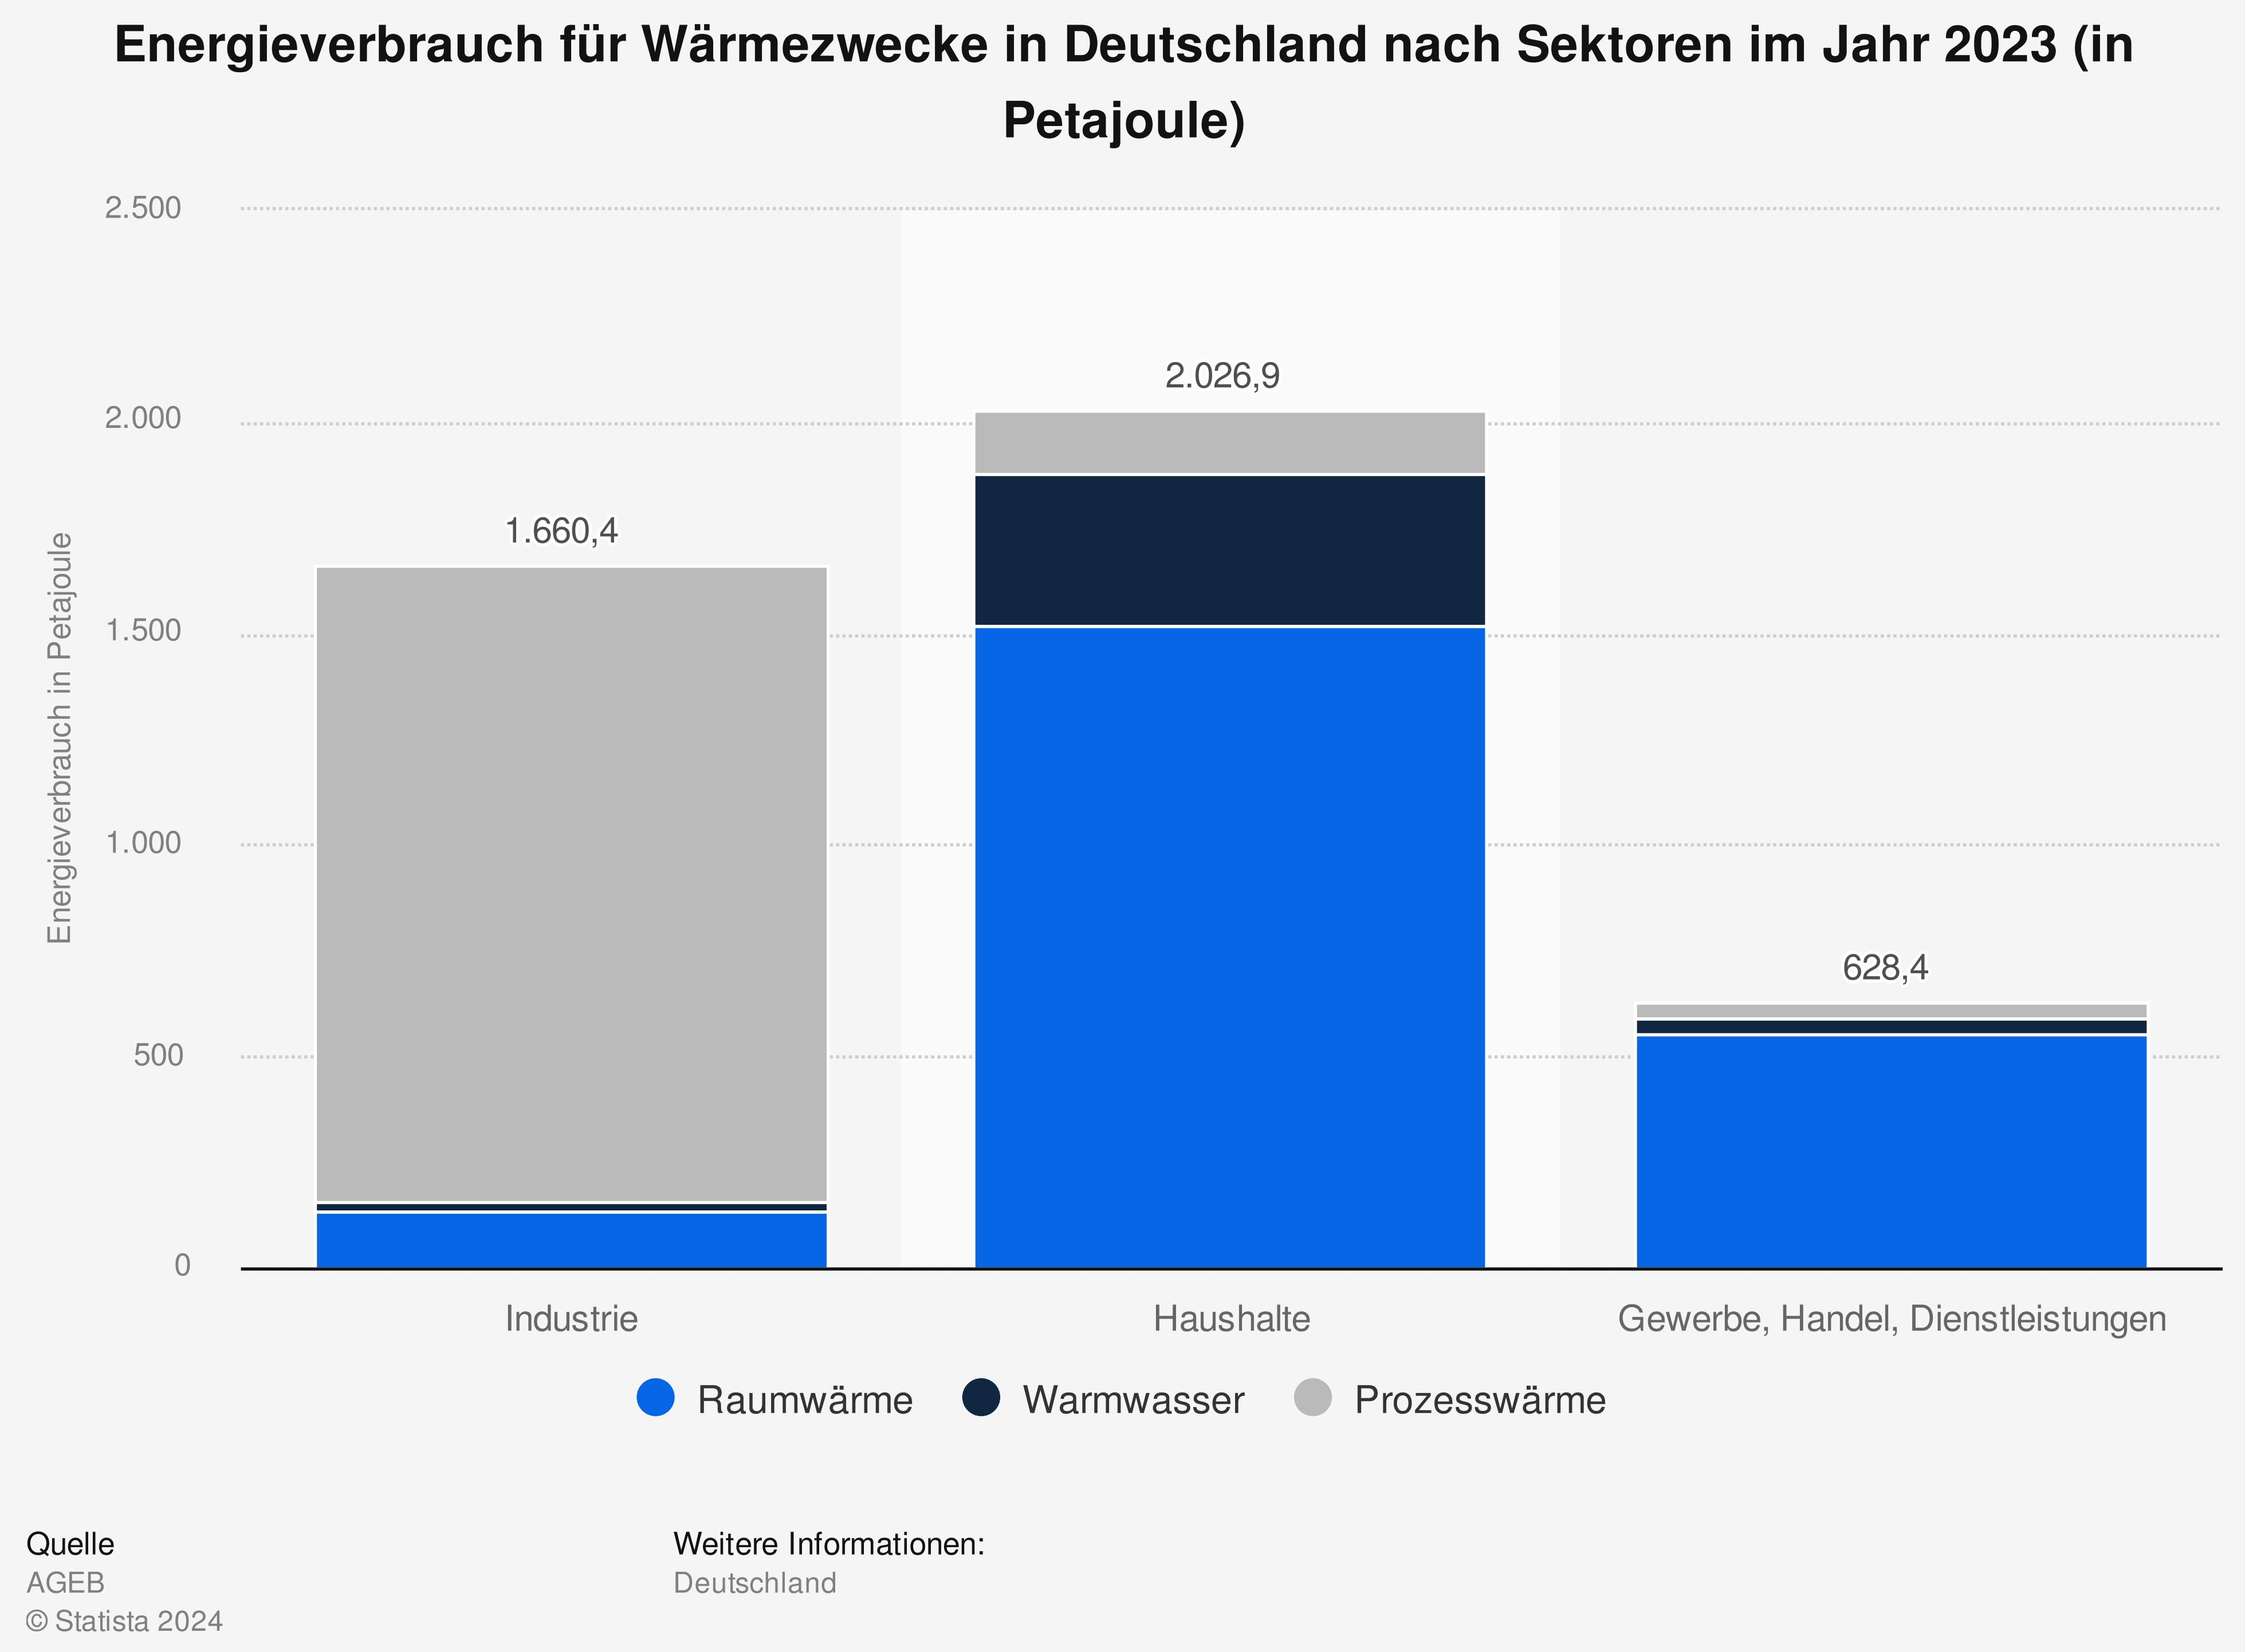
\includegraphics[width=0.68\textwidth]{../../Ressourcen/Bilder/Energieverbrauch_für_Wärmezweck_DE.jpg}
    \caption{Energieverbrauch für den Wärmezweck in Deutschland [\cite{AGEB.2024}]}
    \label{fig:Energieverbrauch_Wärme_DE}
\end{figure}

Die Abbildung \ref{fig:Energieverbrauch_Wärme_DE} zeigt den Energieverbrauch für Wärmezwecke in Deutschland im Jahr 2023, aufgeschlüsselt nach Sektoren. 
Während der industrielle Sektor einen hohen Anteil an prozessbezogener Wärme aufweist, spielt im Dienstleistungssektor die Raumwärme 
eine dominante Rolle.
Diese Statistik bekräftigt die Aussage von Fichera (2020, S. 3) dass bei der Verbesserung der energiebezogenen Leistung in Organisationen des tertiären 
Wirtschaftssektors energiebezogene Prozesse und Technologien im Gegensatz zur Gebäudeenergie eine untergeordnete Bedeutung haben. 

Im Rahmen der Bestimmung des Gesamtenergiebedarfs eines Gebäudes über den Lebenszyklus wird vor allem der Gebäudebetrieb betrachtet (\cite[S. 133]{Musall.2015}).
Die sogenannte Graue Energie wird üblicherweise als kumulierter, nicht erneuerbarer Primärenergieaufwand beschrieben, der alle vor- und nachgelagerten 
Prozesse der verwendeten Baustoffe und Materialien sowie der technischen Anlagen umfasst (\cite[S. 133]{Musall.2015}). Da die DIN EN ISO 50001:2018-12 
auf die fortlaufende Verbesserung der energiebezogenen Leistung abzielt und die Graue Energie konstant ist wird diese im Rahmen dieser Arbeit nicht 
betrachtet. 
Stattdessen liegt der Fokus dieser Forschungsarbeit auf der Bilanzierung energetischer Größen im Rahmen von Organisation des tertiäten Wirtschaftssektors. 
Sie grenzt sich somit von der Bilanzierung von Rohstoffen und Materialien ab.

%%%%%%%%%%%%%%%%%%%%%%%%%%%%%%%%%%%%%%%%%%%%%%%%%%%%%%%%%%%%%%%%%%%%%%%%%%%%%%%%%%%%%%%%%%%%%%%%%%%%%%%%%%%%%%%%%%%%%%%%%%%%%%%%%%%%%%%%%%%%%%%%%%%%%%%%%%%%%%%%%%%

\subsubsection{Definition Bilanzierung}
Im Rahmen des beschrieben Kontexts rückt die verfahrenstechnische Perspektive der Bilanzierung in den Fokus. 
So wird die Bilanzierung im Kontext der Verfahrenstechnik nach Rönsch (2015, S. 66) in drei Bilanzgleichungen unterteilt: 
die Massenbilanz, die Energiebilanz und die Impulsbilanz. 
Zur Beantwortung dieser Forschungsfrage hat insbesondere die Energiebilanz eine hohe Relevanz.

Die Energiebilanz beruht auf dem Energieerhaltungssatz (\cite[S. 66]{Rönsch.2015}), der das Prinzip der Erhaltung 
der Energie ausdrückt (\cite[S. 57]{Baehr.1966}). Der Energieerhaltungssatz bezieht sich auf alle Erscheinungsformen, in denen Energie auftritt, 
und besagt, dass es unmöglich ist, Energie zu erzeugen oder zu vernichten (\cite[S. 57]{Baehr.1966}). 
Für zu bilanzierende Systeme bedeutet dies, dass die Energie in einem abgeschlossenen, adiabaten System über die Zeit 
konstant ist (\cite[S. 66]{Rönsch.2015}). 
Adiabat bedeutet in diesem Kontext, dass das System keine Wärme mit seiner Umgebung austauscht (\cite[S. 66]{Rönsch.2015}). 

Für Systeme, die in der Lage sind, Energie zu speichern, impliziert dies nach Rönsch (2015, S. 66f.), 
dass die darin gespeicherte Energie gleich der Differenz aus ein- und austretenden Energieströmen ist. 
Für offene, nicht-adiabate Systeme ohne Speicherfähigkeit gilt, dass die Differenz der ein- und austretenden Energieströme Null ist 
(\cite[S. 66f.]{Rönsch.2015}).
Das von Rönsch (2015, S. 66f.) beschriebene Verhalten eines Systems bezüglich der Energiespeicherung, lässt sich mathematisch 
vereinfacht mit der Gleichung \eqref{energiebilanzierungsgleichung_Rönsch} darstellen:

\begin{equation}
E_{\text{gespeichert}} = \sum E_{\text{eingang}} - \sum E_{\text{ausgang}}
\label{energiebilanzierungsgleichung_Rönsch}
\end{equation}

\begin{description}
    \item \(E_{\text{gespeichert}}\): Im System gespeicherte Energie.
    \item \(E_{\text{eingang}}\): Energie eines eintretenden Energiestroms.
    \item \(E_{\text{ausgang}}\): Energie eines austretenden Energiestroms.
    \item Für offene, nicht-adiabate Systeme ohne Energiespeicher gilt:
    \[
    E_{\text{gespeichert}} = 0
    \]
    \item In diesem Fall ist die zugeführte Energie gleich der abgegebenen Energie:
    \[
    \sum E_{\text{eingang}} = \sum E_{\text{ausgang}}
    \]
\end{description}

Diese Gleichung beschreibt einen allgemeinen Ansatz zur Energiebilanzierung der im System gespeicherten Energie. 
Im Rahmen der Bilanzierung komplexer Systeme kann jedoch eine detailliertere Bilanzierung einzelner Zustandsgrößen im System erforderlich sein.

Dieses Problem wird von der von Ahrendts (2014, Kapitel 1.5) aufgestellten Bilanzgleichung im Kontext der Thermodynamik addressiert. 
Die Gleichung basiert auf dem Fakt, dass sich für jede mengenartige Zustandsgröße, die über die Grenze eines Systems transportiert wird, eine 
Bilanz aufstellen lässt (\cite[Kapitel 1.5]{Ahrendts.2014}). 
Diese Bilanz umfasst ein- und austretende Ströme sowie im System enthaltene Energiequellen und -senken und ermittelt die 
Geschwindigkeit der Änderung des Bestands der zu bilanzierenden Zustandsgröße im System (\cite[Kapitel 1.5]{Ahrendts.2014}).

Die von Ahrendts (2014, Kapitel 1.5) aufgestellte Bilanzgleichung wird in den Formeln \eqref{BilanzierungsgleichungAhrendt} und 
\eqref{BilanzierungsgleichungAhrendtStrom} dargestellt.

\begin{equation}
    dX_{\text{j}}/d\tau = (\sum \dot{X}_{\text{j,e}} - \sum \dot{X}_{\text{j,a}}) + (\dot{X}_{\text{j,Quell}} - \dot{X}_{\text{j,Senk}})
    \label{BilanzierungsgleichungAhrendt}
\end{equation}

\begin{description}
    \item \(X_{\text{j}}\): Zustandsgröße.
    \item \(\tau\): Zeitintervall.
    \item \(X_{\text{j,e}}\): Über die Systemgrenze zufließende Zustandsgröße.
    \item \(X_{\text{j,a}}\): Über die Systemgrenze abfließende Zustandsgröße.
    \item \(X_{\text{j,Quell}}\): Quellen der Zustandsgröße im System.
    \item \(X_{\text{j,Senk}}\): Senken der Zustandsgröße im System.
\end{description}

Im Rahmen der Formel \eqref{BilanzierungsgleichungAhrendt} wird der Strom einer Zustandsgröße \(X_{\text{j}}\) in Gleichung 
\eqref{BilanzierungsgleichungAhrendtStrom} definiert.

\begin{equation}
    \dot{X}_{\text{j}} = \lim_{\Delta\tau \to 0} \Delta X_{\text{j}}/ \Delta\tau
    \label{BilanzierungsgleichungAhrendtStrom}
\end{equation}

\begin{description}
    \item \(X_{\text{j}}\): Zustandsgröße.
    \item \(\Delta X_{\text{j}}\): Menge der Größe \(X_{\text{j}}\) im Zeitintervall \(\Delta \tau\).
    \item \(\Delta \tau\): Zeitintervall.
\end{description}

Die Gleichung \eqref{BilanzierungsgleichungAhrendt} in Verbindung mit \eqref{BilanzierungsgleichungAhrendtStrom} beschreibt die Geschwindigkeit 
der Änderung des Bestands der Größe \(X_{\text{j}}\) als Summe der Differenzen zwischen den über die Systemgrenze zu- und abfließenden Strömen der 
Zustandsgröße \(X_{\text{j}}\) sowie den Quell- und Senkströmen der Zustandsgröße \(X_{\text{j}}\) innerhalb des Systems.  
Somit formulieren die Gleichungen \eqref{energiebilanzierungsgleichung_Rönsch} und \eqref{BilanzierungsgleichungAhrendt} in Verbindung mit 
\eqref{BilanzierungsgleichungAhrendtStrom} eine grundlegende und zugleich vereinfachte mathematische Beschreibung einer Bilanzierung im Kontext 
der Thermodynamik und Verfahrenstechnik. Sie bilden die Basis für die Beschreibung der grundlegenden Struktur einer Bilanz.
Im Folgenden werden die in \eqref{energiebilanzierungsgleichung_Rönsch} und \eqref{BilanzierungsgleichungAhrendt} mit \eqref{BilanzierungsgleichungAhrendtStrom} 
beschriebenen Bestandteile einer Bilanz zur Konzeption eines Bilanzraums im Anwendungskontext des Problemraums analysiert. 


\subsection{Bilanzräume in der Energiewirtschaft}

%%%%%%%%%%%%%%%%%%%%%%%%%%%%%%%%%%%%%%%%%%%%%%%%%%%%%%%%%%%%%%%%%%%%%%%%%%%%%%%%%%%%%%%%%%%%%%%%%%%%%%%%%%%%%%%%%%%%%%%%%%%%%%%%%%%%%%%%%%%%%%%%%%%%%%%%%%%%%%%%%%%

\subsubsection{Bilanzraumgrenzen zur Abbildung des bilanzierten Systems}
Eine Bilanz bezieht sich gemäß Ahrendts (2014, Kapitel 1.5) auf das von der Systemgrenze eingeschlossene Kontrollgebiet. 
Die Systemgrenze kann dabei unter Berücksichtigung der Zweckmäßigkeit frei definiert werden (\cite[Kapitel 1.5]{Ahrendts.2014}).
Das definierte System kann auch als Bilanzraum bezeichnet werden, da die Berechnung der in einen Bilanzraum ein- und austretenden Ströme als Bilanzierung bezeichnet wird (\cite[S. 65]{Rönsch.2015}).
Einen Ansatz zur Definition von Bilanzräumen liefert Miller (2016, S. 105) mit der Konkretisierung von Bewertungsräumen mittels Kriterien der Bilanzgrenze, dem 
Aggregationsniveau und der Bewertungseinheit. Das definierte System Dient der Bewertung der Nutzung der Ressourcen wobei der Effizienzbegriff eine zentrale Rolle spielt (\cite[S. 107]{Miller.2016}).
Miller (2016, S. 107) definiert die Effizienz nach Gleichung \eqref{EffizienzgleichungMiller}.

\begin{equation}
    \text{Effizienz} := \frac{\text{Erreichter Nutzen}}{\text{Aufwand}}
    \label{EffizienzgleichungMiller}
\end{equation}

Der Aufwand umfasst nach Miller (2016, S. 108f.) unterschiedliche Ressourcen, wobei im Kontext energiewirtschaftlicher Fragestellungen der Fokus auf der Ressource Energie 
liegt.
Der Nutzen ist vom Untersuchungsgegenstand abhängig und wird im Kontext der energiewirtschaftlichen 
Fragestellung häufig über Energiedienstleitstungen operationalisiert (\cite[S. 107]{Miller.2016}). Betrachtet man dass der Nutzen grundsätzlich durch Befriedigung 
von Bedürfnissen beschrieben wird entsteht im Kontext der Energiewirtschaft ein Nutzenergiebedarf zur Befriedigung der Bedürfnisse im Rahmen einer Energiedienstleitstung 
(\cite[S. 107]{Miller.2016}). 
Sowohl die Ressourcen des Aufwands als auch die Energiedienstleistung auf Nutzenseite werden durch eine Bewertungseinheit formalisiert (\cite{Miller.2016}).
Der Nutzen wird meist implizit durch den gewählten Untersuchungsgegenstand definiert (\cite[S. 110]{Miller.2016}).
Die in \eqref{EffizienzgleichungMiller} aufgestellte Nutzen-Aufwand Relation stellt die Grundlage der Definition der Bilanzraumgrenze dar. 
Die Bilanzraumgrenze lässt sich somit in die Aufwandsseitige Bilanzgrenze, die alle zu bilanzierenden Ressourcen umfasst und die Nutzenseitige Bilanzrgrenze die sich auf 
die zu Bilanzierende Energiedienstleitstung bezieht (\cite[S. 111]{Miller.2016}).  

Das von Miller (2016) beschriebene Konzept bringt eine neue Perspektive auf die in \eqref{BilanzierungsgleichungAhrendt} und \eqref{BilanzierungsgleichungAhrendtStrom} 
aufgestellte Bilanzgleichung. Sie bringt das Prinzip der Effizienz ein und teilt eine Bilanz in Aufwands und Nutzenseite. 
Aufwandsseitig sind die in \eqref{BilanzierungsgleichungAhrendt} zufließenden Ströme, also die dem System zugeführten Ressourcen der Zustandsgröße zu betrachten. 
Nutzenseitig müssen abfließende Ströme, also die aus dem System fließende Energie zur Befriedigung der Energiedienstleistung der Zustandsgröße betrachtet werden. 
Die abfließenden Ströme werden nach Energiedienstleistung mit Nutzengrößen operationalisiert (\cite{Miller.2016}).

%%%%%%%%%%%%%%%%%%%%%%%%%%%%%%%%%%%%%%%%%%%%%%%%%%%%%%%%%%%%%%%%%%%%%%%%%%%%%%%%%%%%%%%%%%%%%%%%%%%%%%%%%%%%%%%%%%%%%%%%%%%%%%%%%%%%%%%%%%%%%%%%%%%%%%%%%%%%%%%%%%%

\subsubsection{Zustandsgrößen, Nutzengrößen und Nutzenergiebedarf}
In einem Thermodynamischen System wird der augenblickliche Zustand durch die Zustandsgrößen beschrieben, wobei diese in intensive und extensive Zustandsgrößen 
unterschieden werden (\cite[S. 66]{Konstantin.2023}). Die innere Energie U ist eine extensive Zustandsgröße (\cite[S. 65]{Konstantin.2023}), und rückt in den 
Fokus da es sich um eine energetische Zustandsgröße handelt. Das Verhalten einer Zustandsgröße ist in \eqref{BilanzierungsgleichungAhrendt} und \eqref{BilanzierungsgleichungAhrendtStrom} 
beschrieben.

In dieser Forschung bezieht sich der Untersuchungsgegenstand aufgrund der verortung der Organisationen im tetriären Wirtschaftssektors auf Gebäudeenergie. 
Es müssen also auf der Grundlage dieses Untersuchungsgegenstands angemessene Nutzengrößen mit entsprechenden Bewertungseinheiten erfasst werden. 
Da auch die Definition der Systemgrenze vom Untersuchungsgegenstand beeinflusst wird (\cite[S. 109]{Miller.2016}) gilt die Zweckmäßigkeit der Systemgrenze 
auch für die zu untersuchenden Nutzengrößen.
Die DIN EN ISO 50001:2018-12 gibt mit dem Ziel der fortlaufenden Verbesserung der energiebezogenen Leistung eine Vorgabe zur zweckmäßigen Definition der Nutzengröße 
(\cite[S. 11]{DIN50001.2018}).
Die Vornorm DIN V 18599-1:2018-09, herausgegeben vom Deutschen Institut für Normung e. V. (2018, S. 1), behandelt die energetische Bewertung von Gebäuden und stellt ein 
Verfahren zur Durchführung der Gesamtenergiebilanz bereit (\cite[S. 9]{DIN18599.2018}). Ihre Ausrichtung auf die energetische Bewertung erfüllt die Zweckmäßigkeit der 
DIN EN ISO 50001:2018-12. Der Fokus auf die Bewertung von Gebäuden entspricht der Zielsetzung der DIN V 18599-1:2018-09. 

Im Rahmen der energetischen bewertung von Gebäuden betrachtet die DIN V 18599-1:2018-09 die Bilanzierung des Nutz-, End- und Primärenergiebedarf (\cite{DIN18599.2018}).
In einem energiewirtschaftlichen Rahmen hat besonders der Nutzeenergiebedarf eine Große Bedeutung da er aus der Befriedigung der Bedürfnisse im Rahmen einer 
Energiedienstleistung resultiert (\cite[S. 107]{Miller.2016}).

\begin{figure}[H]
    \centering
    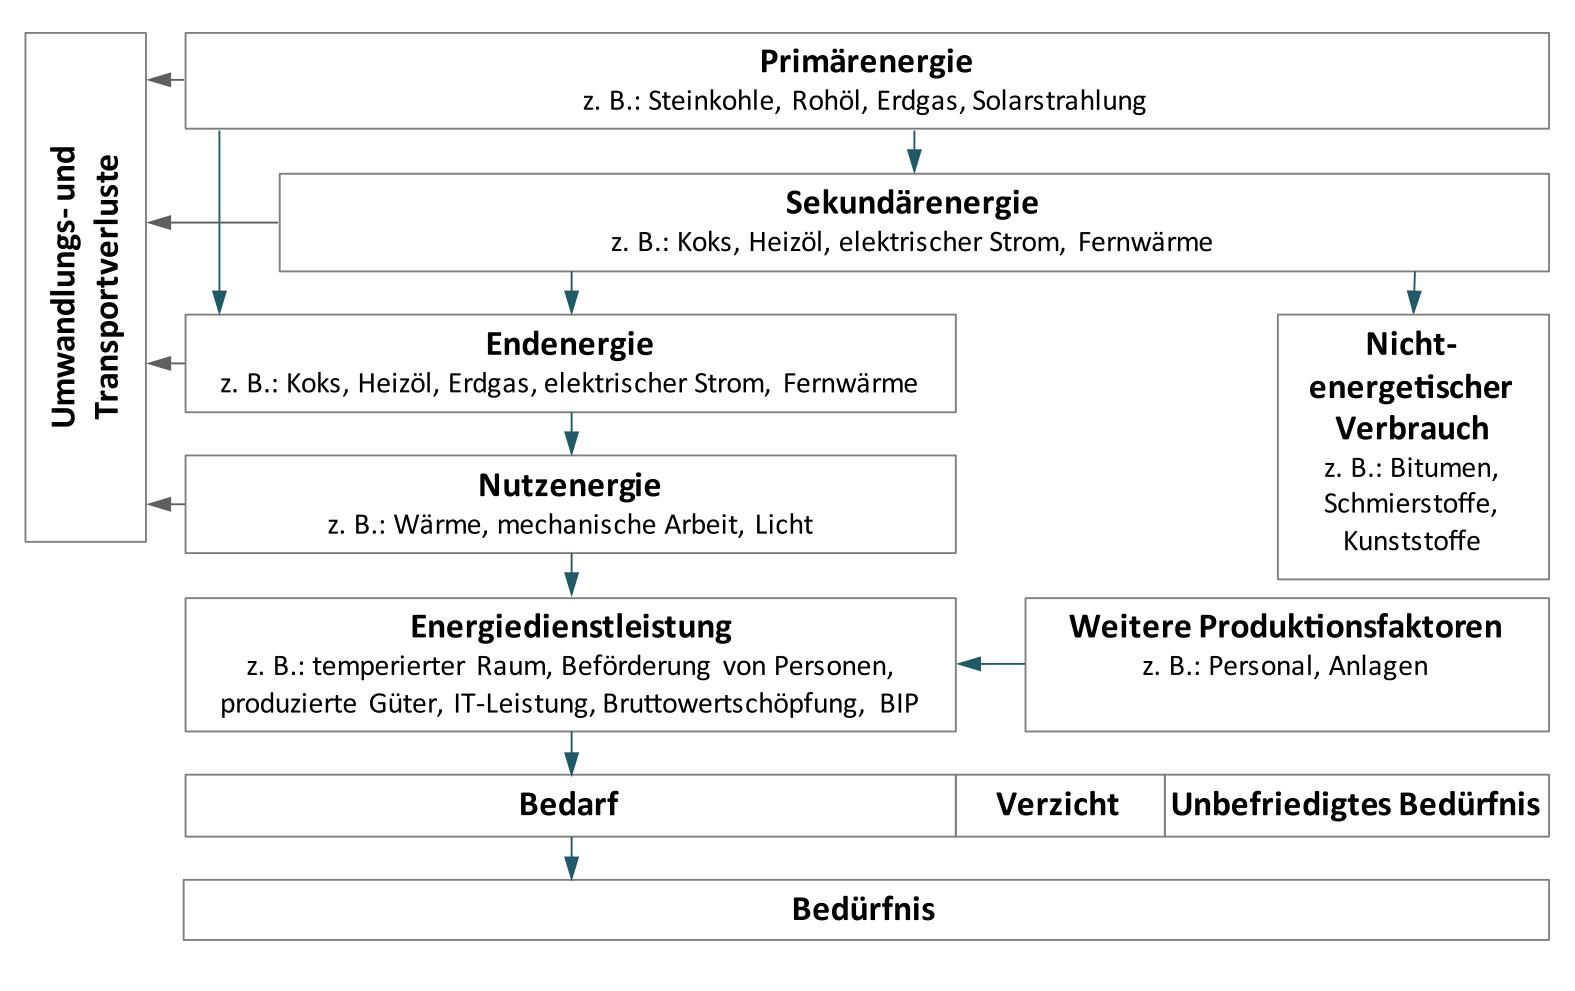
\includegraphics[width=0.8\textwidth]{../../Ressourcen/Abbildungen/Energiefluss_Miller.jpg}
    \caption{Energieflussschema. (Dargestellt von Miller (2016))}
    \label{fig:Energieflussschema_Miller}
\end{figure}

Im Energieflussdiagramm \eqref{fig:Energieflussschema_Miller} wird die Nutzenergie zwischen der Endenergie und der Energiedienstleistungen verortet. 
Da die Endenergie die Energiemenge ist, die dem Bilanzraum zur bestimmungsgemäßen Nutzung bereitgestellt wird (\cite[Kapitel 3.1.2]{DIN18599.2018}), 
Repräsentiert diese Energieform die Menge der potentiellen Ressourcen auf Aufwandsseite der Bilanzierung.
Außerdem wird der praktische Sachverhalt veranschaulicht dass bei der Umwandlung von Endenergie in Energiedienstleistungen über die Nutzenergie 
Umwandlungs und Transportverluste berücksichtigt werden müssen.

Die DIN V 18599-1:2018-09 definiert die Heizung, Kühlung, Lüftung, Trinkwarmwasseraufbereitung und Beleuchtung von Gebäuden oder Gebäudezonen 
als relevante Nutzengrößen zur energetischen Bewertung von Gebäuden (\cite{DIN18599.2018}). 
Somit wird im von Miller (2016) aufgestellten Konzept der Nutzenergiebedarf der jeweiligen Nutzengröße durch die Nutzenergie gedeckt, 
und muss je nach Nutzengröße unterschiedlich definiert werden. Die Nutzenergie wird im Konzept von Miller (2016) durch die Ressourcen repräsentiert.
Im Rahmen der Vornorm wird der Nutzenergiebedarf als Überbegriff für Nutzwärmebedarf, Nutzkältebedarf, Nutzenergiebedarf für Tinkwarmwasser, Beleuchtung und 
Befeuchtung definiert (\cite[Kapitel 3.1.3]{DIN18599.2018}).
Der Nutzenergiebedarf der Beleuchtung ist definiert als rechnerisch ermittelter Energiebedarf, der sich ergibt, wenn die Gebäudezone mit der im Nutzungsprofil 
festgelegten Beleuchtungsqualität beleuchtet wird (\cite[Kapitel 3.1.6]{DIN18599.2018}). 
Analog dazu versteht sich die Nutzeenergie für die Beleuchtung als die Energiemenge die zur Ausreichenden Beleuchtung der Gebäudezone aufgewendet werden muss (\cite[Kapitel 5.3.1]{DIN18599.2018}).
Der Nutzwärmebedarf hingegen ist der rechnerisch ermittelter Wärmebedarf, der zur Aufrechterhaltung der festgelegten thermischen Raumkonditionen innerhalb einer Gebäudezone während der Heizzeit benötigt wird
rechnerisch ermittelter Energiebedarf, der sich ergibt, wenn die Gebäudezone mit der im Nutzungsprofil festgelegten Beleuchtungsqualität beleuchtet wird(\cite[Kapitel 3.1.4]{DIN18599.2018}).
Der Nutzkältebedarf ist der rechnerisch ermittelter Kühlbedarf, der zur Aufrechterhaltung der festgelegten thermischen Raumkonditionen innerhalb einer Gebäudezone benötigt wird in Zeiten, 
in denen die Wärmequellen eine höhere Energiemenge anbieten als benötigt wird(\cite[Kapitel 3.1.5]{DIN18599.2018}).
Die Wärmeenergie ist die Wämemenge, die der Gebäudezone zusätzlich (bedarfs-)geregelt zugeführt werden muss, um die vorgegebene 
Sollinnentemperatur einzuhalten (\cite[Kapitel 5.3.1]{DIN18599.2018}).
Der Nutzenergiebedarf für die Trinkwarmwasserbereitung ist definiert als der rechnerisch ermittelte Kühlbedarf, der zur Aufrechterhaltung der festgelegten thermischen Raumkonditionen innerhalb einer Gebäudezone benötigt wird in Zeiten, in denen die Wärmequellen eine höhere Energiemenge anbieten als benötigt wird
rechnerisch ermittelter Energiebedarf, der sich ergibt, wenn die Gebäudezone mit der im Nutzungsprofil festgelegten Menge an Trinkwarmwasser entsprechender Zulauftemperatur versorgt wird (\cite[Kapitel 3.1.7]{DIN18599.2018}).
Die Nutzenergie für die Trinkwarmwasserbereitung bedeutet die Energiemenge für die Erwärmung des Trinkwassers von der Kaltwassertemperatur auf die 
Warmwassertemperatur an der Entnahmestelle (\cite[Kapitel 5.3.1]{DIN18599.2018}).
Im Rahmen der Luftaufbereitung versteht sich die Nutzenergie als Energiemenge die zum Erwärmen, Kühlen, Befeuchten und Entfeuchten der Luft in einer 
raumlufttechnischen Anlage zu- beziehungsweise abgeführt werden muss um den erforderlichen Zuluftzustand zu erreichen (\cite[Kapitel 5.3.1]{DIN18599.2018}).

Abbildung \eqref{fig:Übersicht_Bilanzräume} Ordnet den mithilfe der DIN V 18599-1:2018-09 erfassten Untersuchungsgegenstand in das von Miller (2016) erarbeitete Konzept der 
Bewertungsräume ein.

\begin{figure}[H]
    \centering
    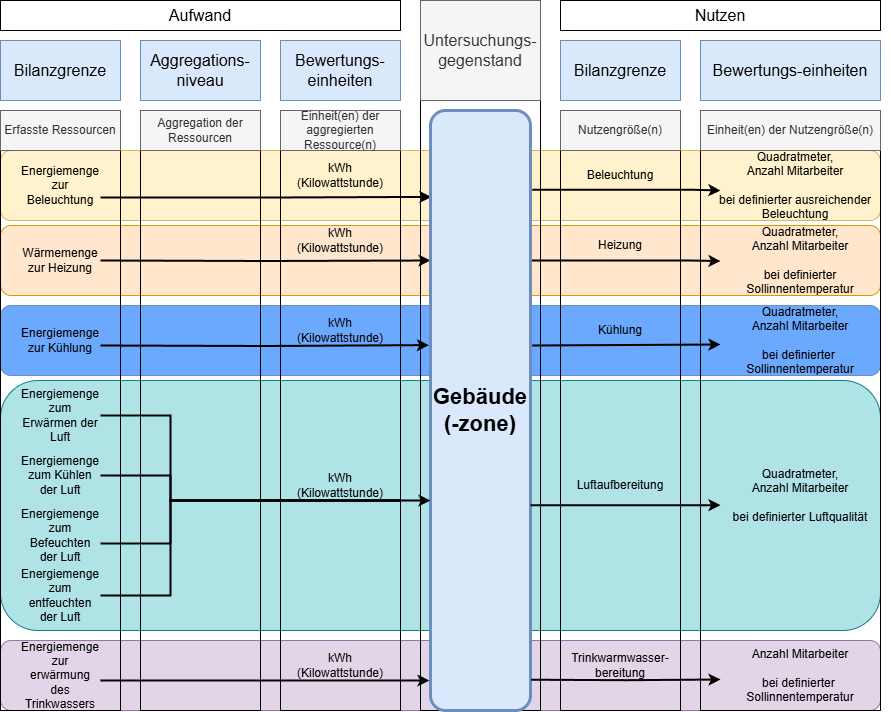
\includegraphics[width=1\textwidth]{../../Ressourcen/Abbildungen/Nutzengröße_Bewertungseinheit.png}
    \caption{Übersicht Bilanzräume. (Eigene Darstellung basierend auf Miller (2016) und DIN V 18599-1:2018-09 (2018))}
    \label{fig:Übersicht_Bilanzräume}
\end{figure}

%%%%%%%%%%%%%%%%%%%%%%%%%%%%%%%%%%%%%%%%%%%%%%%%%%%%%%%%%%%%%%%%%%%%%%%%%%%%%%%%%%%%%%%%%%%%%%%%%%%%%%%%%%%%%%%%%%%%%%%%%%%%%%%%%%%%%%%%%%%%%%%%%%%%%%%%%%%%%%%%%%%

\subsubsection{Energieströme und Bewertungseinheiten}
In der Gleichung \eqref{BilanzierungsgleichungAhrendtStrom} wird der Strom einer Zustandsgröße als Menge der Zustandsgröße in einem infinitesimal kleinen Zeit-
intervall definiert, welches im Grenzwert gegen 0 geht. Folglich wird ein Strom von Ahrendts (2014) als Menge einer Zustandsgröße zu einem bestimmten Zeitpunkt 
definiert. 

In Gleichung \eqref{BilanzierungsgleichungAhrendt} wird zwischen in das System zu- und abfließende Ströme der Zustandsgröße Unterschieden.
Die zufließenden Ströme können als Ressourcen der Aufwandsseite im von Miller (2016) aufgestellten Konzept der Bewertungsräume betrachtet werden, 
wobei energetische Ressourcen im Vordergrund stehen. Aufwandsseitige Ressourcen können zu einer Ressource mit einer Bewertungseinheit 
zusammengefasst werden (\cite[S. 112]{Miller.2016}). Sollten nach erfassung und optionaler aggregation der Ressourcen mehrere Ressourcenkategorien bestehen, 
können diese mit unterschiedlichen Bewertungseinheiten bilanziert werden (\cite[S. 112]{Miller.2016}). Im Rahmen dieser Forschungsarbeit werden 
Aufwandsseitig jedoch ausschließlich Energieressourcen betrachtet.
Sie Stammen somit aus dem Bereich der Endenergie und haben die Bewertungseinheit: kWh und deren Vielfaches da diese Einheit bei Energiebilanzen in der Regel für alle 
Energieformen bevorzugt verwendet wird (\cite[S. 65]{Konstantin.2023}).

Die abfließenden Ströme in \eqref{BilanzierungsgleichungAhrendt} repräsentieren die Nutzenseite des von Miller (2016) aufgestellten Konzepts.
Um die Nutzenseite abzubilden ist eine Konkretisierung der Energiedienstleistung durch eine angemessene Bewertungseinheit, 
welche vom Untersuchungsgegenstände impliziert wird notwendig (\cite{Miller.2016}). Diese Bewertungseinheit ist keine Energieeinheit, und 
kann beispielsweise bei der Untersuchung der Temperierung von Räumen die Quadratmeteranzahl des Bilanzraums bei einer definierten 
soll Temperierung sein (\cite{Miller.2016}). 

Eine praktische Herausforderung im Rahmen der Bilanzierung ist die Energiedatensammlung der zu erfassenden Ströme zu der auch die DIN EN ISO 50001:2018-12 vorgaben macht. 
Die DIN EN ISO 50001:2018-12 (2018, Kapitel 6.6, A.6.6) stellt Anforderungen und Qualitätskriterien an die Datensammlung in Organisationen.
Diese verpflichtet Organisationen dazu Hauptmerkmale ihrer Tätigkeiten, die sich auf die energiebezogene Leistung auswirken zu identifizieren, und diese in geplanten 
Zeitabständen zu messen, überwachen und analysieren (\cite[S. 23]{DIN50001.2018}).
Teil der zu erfassenden Hauptmerkmale sind relevante Variablen bezüglich wesentlicher Energieeinsätze, den Energieverbrauch bezüglich wesentlicher Einsätze 
und der Organisation und betriebliche Kriterien bezüglich wesentlicher Energieeinsätze(\cite[S. 23]{DIN50001.2018}).
Die komplexität der Umsetzung ist dabei nicht vorgeschrieben und kann von einfachen Zählwerten bis hin zu umfangreichen Werten aus Überwachungs- und Messystemen mit 
Softwareandwendung reichen (\cite[S. 36]{DIN50001.2018}).

%%%%%%%%%%%%%%%%%%%%%%%%%%%%%%%%%%%%%%%%%%%%%%%%%%%%%%%%%%%%%%%%%%%%%%%%%%%%%%%%%%%%%%%%%%%%%%%%%%%%%%%%%%%%%%%%%%%%%%%%%%%%%%%%%%%%%%%%%%%%%%%%%%%%%%%%%%%%%%%%%%%

\subsubsection{Energiequellen und -senken}
Gleichung \eqref{BilanzierungsgleichungAhrendt} unterscheidet zwischen Quellen, Senken und zu- beziehungsweise abfließenden Strömen der Zustandsgröße. 
Quell- und Senkenströme treten in einer Energiebilanz nach dem ersten Hauptsatz der Thermodynamik nicht auf da Energie als Erhaltungsgröße ist (\cite[S. 14]{Ahrendts.2014}). 
Im Rahmen der DIN EN ISO 50001:2018-12 bezieht sich der Begriff Energie auf verschiedene Arten von Energie die erworben, gespeichert, aufbereitet, in einer Einrichtung oder einem Prozess verwendet 
oder zurückgewonnen werden können (\cite[Kapitel 3.5.1]{DIN50001.2018}). Energie kann im Rahmen der Norm als Elektrizität, Brennstoff, Dampf, Wärme, Druckluft oder vergleichbares Medium auftreten 
(\cite[Kapitel 3.5.1]{DIN50001.2018}).
Folglich werden alle Energieströme, in denen Energie in eine Energieform umgewandelt wird, die nicht die genannten Kirterien erfüllen als Energiesenken betrachtet. 
Analog dazu werden alle Energieströme, bei denen Energie, die nicht den von der Norm aufgestellten Kriterien entspricht, in eine nach ISO 50001 definierte Energieform 
umgewandelt wird, als Energiequellen betrachtet.
In der Praxis stellen die in Abbildung \eqref{fig:Energieflussschema_Miller} dargestellten Umwandlungs- und Transportverluste Energiesenken dar. Energiequellen können beispielsweise 
PV-Anlagen sein, da diese die Energie des Sonnenlichts, welche nach Definition der DIN EN ISO 50001:2018-12 nicht Nutzbar ist in nutzbare Energie umwandelt und als 
Endenergie zur Verfügung steht.

\subsubsection{Bilanzraumstrukturen}
Bisher wurde die strukturelle Definition von Bilanzräumen unter anbetracht praktischer Herausforderung unter der DIN EN ISO 50001:2018-12 in Organisationen 
des tertiären Wirtschaftssektors betrachtet. Allerdings können auch zwischen Bilanzräumen Beziehungen bestehen, welche im folgenden erläutert werden.

Ein Bilanzraum kann in mehrere Teilbilanzräume zerlegt werden (\cite[S. 310]{Engelmann.2015}). Dies kann durch die Zerlegung in einzelne Prozesse, 
Anlagen oder Räumlich getrennte Bereiche realisiert werden (\cite[S. 310]{Engelmann.2015}), wobei die Zerlegung in Prozesse bei Organisationen des tertiären 
Wirtschaftssektors eine geringere Relevanz hat.
Analog zur Zerlegbarkeit eines Bilanzraums lässt sich auch der Untersuchungsgegenstand eines Bilanzraums Hierarchisch aufgliedern (\cite[S. 109]{Miller.2016}).

Zur Erfassung der Energiedaten einer Organisation bedarf es eine detaillierte und aussagekräftige Analyse der Unterscheidung nach Verbrauchsarten 
(\cite[S. 14]{Hohnhold.2013}). Dabei ist die Disagggregation der Daten von der Größe der Organisation und dem Zweck der Analyse möglich (\cite[S. 14f.]{Hohnhold.2013}).
Die beschriebene Unterscheidung nach Verbrauchsarten kann durch die Zerlegung eines Bilanzraums mit mehreren Nutzengrößen in Bilanzräume mit einer Nutzengröße 
realisiert werden. Da die DIN V 18599-1:2018-09 Gebäude in Zonen, welche als grundlegende räumliche Berechnungseinheit für die Energiebilanzierung definiert sind (\cite[Kapitel 3.1.12]{DIN18599.2018}), 
unterteilt, ist auch eine Zerlegung des Untersuchungsgegenstands in einzelne Gebäudezonen Sinnvoll.

\section{Energiemanagement nach ISO 50001}

\subsection{Bewertung der Energiebezogenen Leistung}
\subsubsection{Definition von Energieleistungskennzahlen}
Im Rahmen der Planungsphase des PDCA-Zyklus verpflichtet die DIN EN ISO 50001:2018-12 Organisationen zur Festlegung von Energieleistungskennzahlen 
(\cite[S. 7]{DIN50001.2018}).
Eine Energieleistungskennzahl, auch EnPi (en: energy performance indicator) gennant, ist ein Maß oder eine Einheit der energiebezogenen Leistung, wie Sie von der Organisation festgelegt ist 
(\cite[Kapitel 3.4.4]{DIN50001.2018}), und ist somit ein Maßstab für den Vergleich der energiebezogenen Leistung (\cite[Kapitel A.6.4]{DIN50001.2018}). 
Eine Energieleistungskennzahl wird durch einen EnPI-Wert zu einem bestimmten Zeitpunkt oder über einen bestimmten Zeitraum quantifiziert (\cite[Kapitel 3.4.5]{DIN50001.2018}).
EnPI-Werte finden Verwendung in der gesamten Organisation und in verschiedenen Teilen der Organisation (\cite[S. 13]{DIN50006.2024}). 
EnPIs ermöglichen einen Vergleich zwischen unterschiedlichen Untersuchungsgegenständen, können zeitliche Veränderungen der energiebezogenen Leistung darstellen und dienen als 
Zielvorgaben und zur Erfolgskontrolle (\cite[S. 2]{Hohnhold.2013}).
Sie bilden nach Hohnhold (2013, S. 2) den Mittelpunkt jeder Bewertung von Energieeffizienz und verdichten Informationen über den Energieverbrauch und dessen Struktur in einer 
Organisation. 
Folglich bilden EnPIs und EnPI-Werte die Grundlage der energiebezogenen Leistung und deren Verbesserung, und sind somit eine Eingangsgröße für die Managementbewertung der energiebezogenen Leistung 
in der Prüfungsphase des PDCA-Zyklus (\cite[Kapitel 9.3.3]{DIN50001.2018}).

Energieleistungskennzahlen hängen mit energetischen Ausgangsbasen zusammen und können Organisationen in die Lage versetzen eine Verbesserung der energiebezogenen Leistung, anhand von verbesserungen bei EnPI-Werten 
im zeitlichen Verlauf im Verhältnis zur entsprechenden energetischen Ausgangsbasis, nachzuweisen (\cite[Kapitel 0.3]{DIN50001.2018}).
Eine Energetische Ausgangsbasis, auch EnB (en: energy baseline) ist von der DIN EN ISO 50001:2018-12 definiert als quantifizierbarer(e) Referenzpunkt(e) für einen Vergleich der energiebezogenen 
Leistung und beruht auf Daten aus einem festgelegten Zeitabschnitt und/oder auf Bedingungen wie von der Organisation festgelegt(\cite[Kapitel 3.4.7]{DIN50001.2018}). 

\begin{figure}[H]
    \centering
    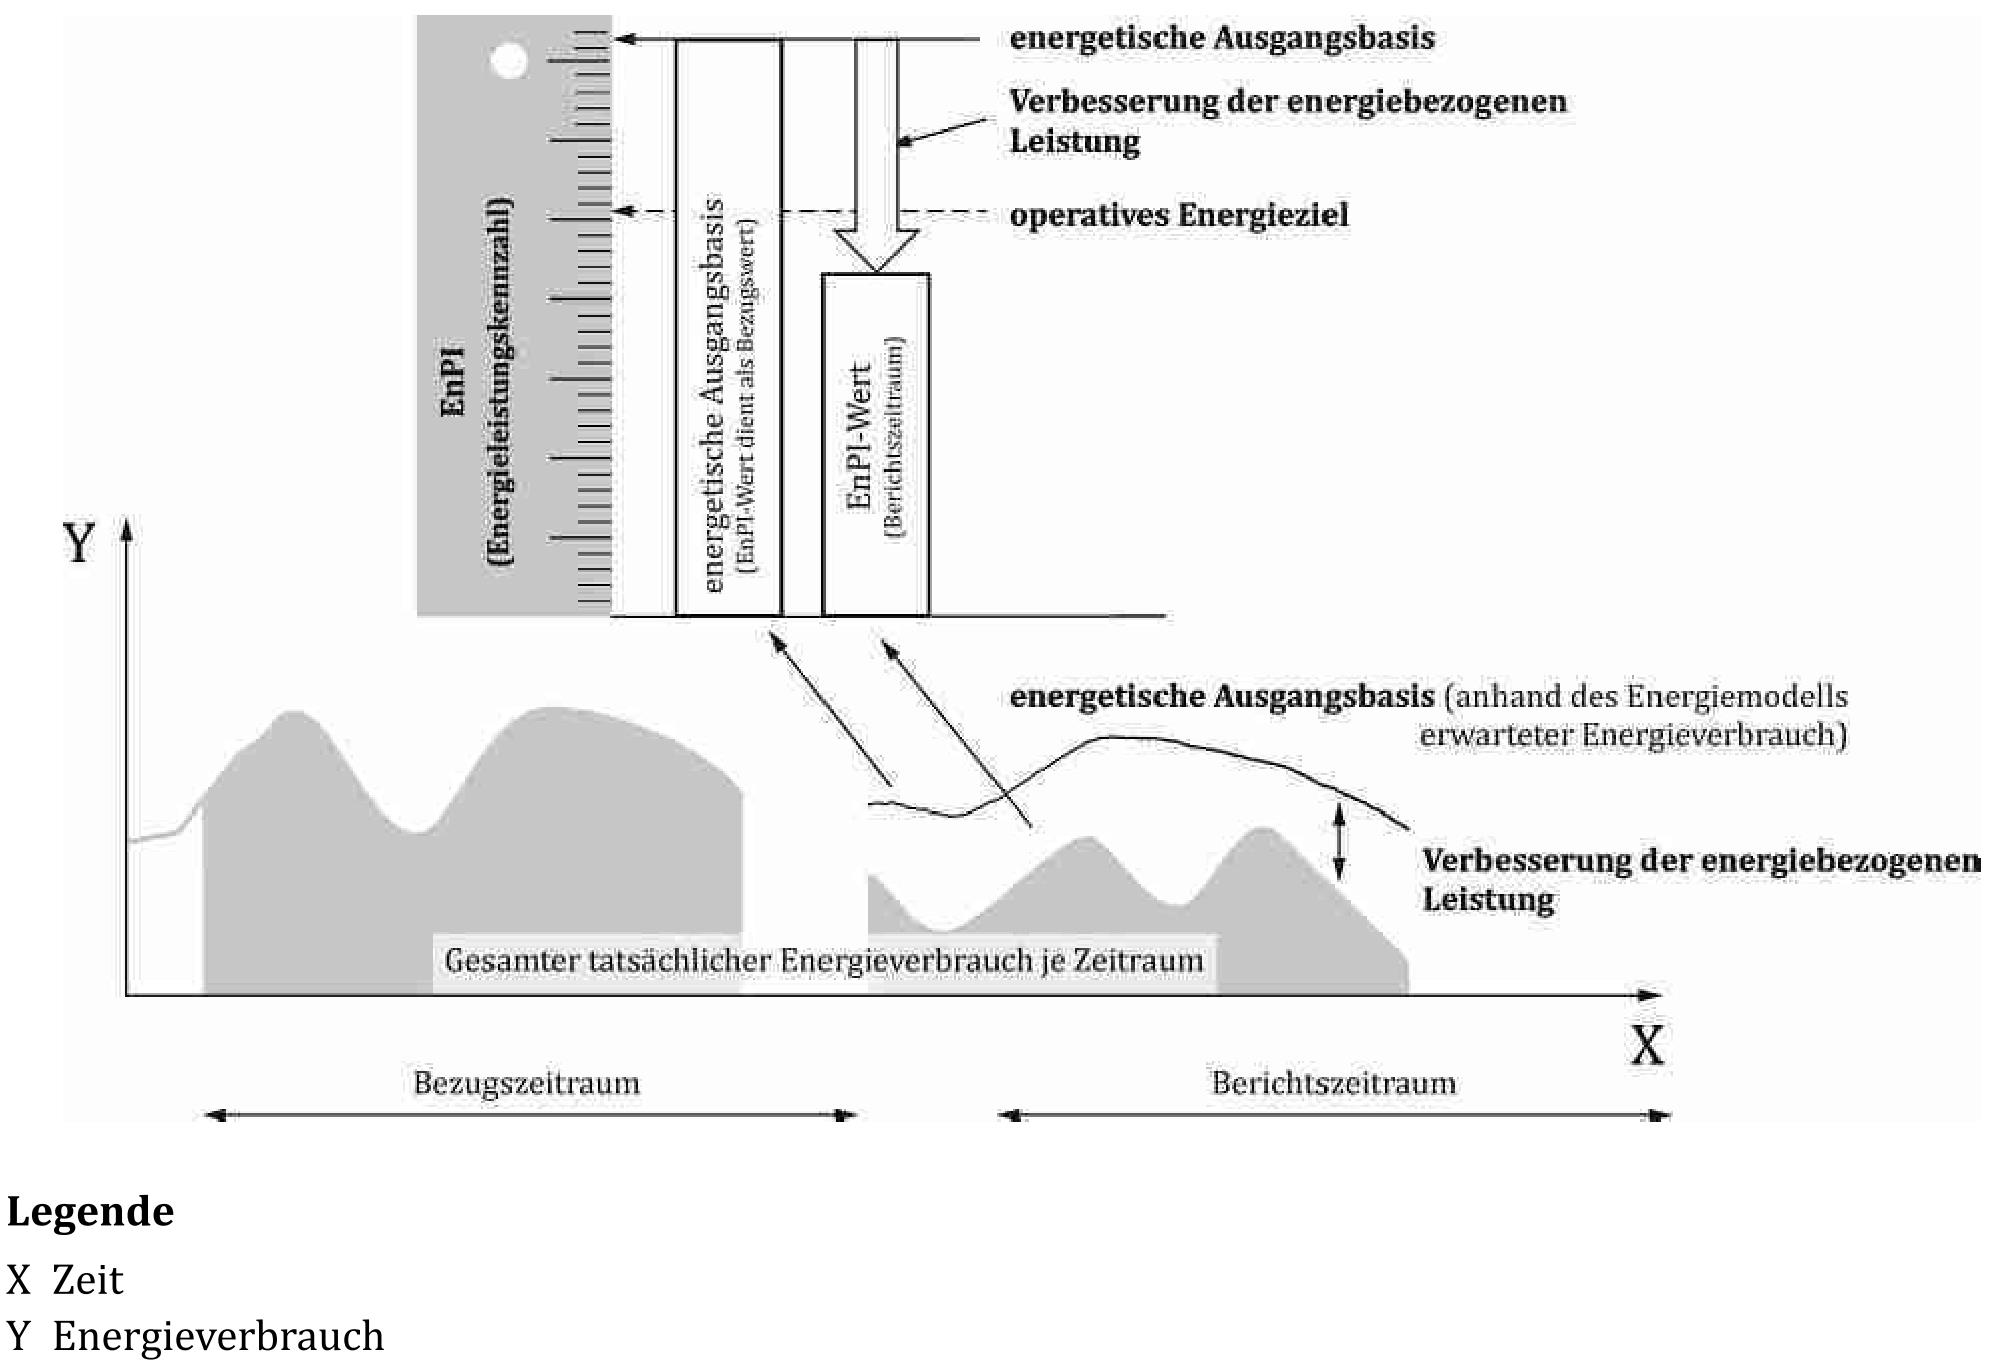
\includegraphics[width=1\textwidth]{../../Ressourcen/Abbildungen/ISO_50006_Beispiel_EnPI_EnB.jpg}
    \caption{Beispiel für die konzeptuelle Beziehung zwischen der energiebezogenen Leistung, EnPIs, EnBs, EnPI-Werten und operativen Energiezielen. (Darstellung der E DIN ISO 50006:2024-07 (2024, S. 14))}
    \label{fig:Beziehung_EnPI_EnB_ISO_50006}
\end{figure}

Die E DIN ISO 50006:2024-07 zeigt ein Beispiel für die Beziehungen zwischen der energiebezogenen Leistung, EnPIs, EnBs, EnPI-Werten und operativen Energiezielen 
in Abbildung \eqref{fig:Beziehung_EnPI_EnB_ISO_50006} auf.
Hier wird der Energieverbrauch über einen Berichtszeitraum, als Energieleistungskennzahl definiert.
Die energetische Ausgangsbasis stellt anhand des Energiemodells den erwarteten Energieverbrauch.
Das operative Energieziel gibt den Zielwert des EnPI-Werts im Berichtszeitraum an. 
Die differenz zwischen dem EnB den EnPI-Werten ergibt die Verbesserung der Energiebezogenen Leistung.
Neben der Auskunft über die relevanten Bestandteile zum Nachweis der energiebezogenen Leistung, gibt das Beispiel (vgl. Abbildung \eqref{fig:Beziehung_EnPI_EnB_ISO_50006}) 
zwei Perspektiven auf die Auswertung der genannten Komponenten.
So wird in der unteren Visualisierung die Verbesserung der energiebezogenen Leistung über einen Berichtszeitraum in einem Zeit-Energieverbrauch-Graphen dargestellt.
Diese Art der Visualisierung ermöglicht Erkenntnisgewinne bezüglich des Zeitabhängigen Verhaltens des EnPI-Werts und kann unter anderem zur Identifkation des 
einflusses zeitabhängiger relevanter Variablen wie saisonaler Wetterbedingungen genutzt werden. 
Die Obere Visualisierung aggregiert die EnPI-Werte und die EnB über den Berichtszeitraum zu einzelnen Werten. 
Anhand dieser Werte kann die Erfüllung oder nicht-Erfüllung des operativen Energieziels im Berichtszeitraum evaluiert werden.

\subsubsection{Arten von Kennzahlen aus statistisch-methodischer Perspektive}

\begin{figure}[H]
    \centering
    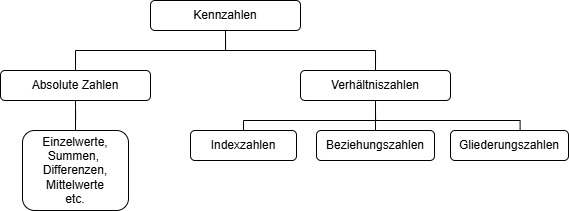
\includegraphics[width=1\textwidth]{../../Ressourcen/Abbildungen/Arten_von_Kennzahlen.jpg}
    \caption{Arten von Kennzahlen. (Eigene Darstellung basierend auf Hohnhold (2013, S. 4))}
    \label{fig:Arten_Kennzahlen}
\end{figure}

Grundsätzlich lassen sich Kennzahlen aus statistisch-methodischer Sicht in zweit Klassen unterteilen: absolute Zahlen und Verhältniszahlen (vgl. Abbildung \eqref{fig:Arten_Kennzahlen}).
Absolute Zahlen werden durch Einzelwerte, Summen, Differenzen oder Mittelwerten abgebildet und eignen sich aufgrund der absoluten Betrachtung auf Aufwandsseite nicht zur Bewertung der Energieeffizienz (\cite[S. 2]{Hohnhold.2013}).
So fällt auch der im oberen Teil der Abbildung \eqref{fig:Beziehung_EnPI_EnB_ISO_50006} dargestellte über den Berichtszeitraum aggregierte Energieverbrauch 
in die Klassifizierung einer absoluten Kennzahl (\cite[S. 2]{Hohnhold.2013}).
Obwohl absolute Zahlen nicht zur Bewertung der Energieeffizienz geeignet sind, können sie wie in Abbildung \eqref{fig:Beziehung_EnPI_EnB_ISO_50006} visualisert 
auskunft über die Verbesserung der energiebezogenen Leistung geben.

Verhältniszahlen bilden einen Quotienten aus zusammenhängenden Größen und sind dadurch besser zur Analyse der Energieeffizienz geeignet (\cite[S. 3]{Hohnhold.2013}).
Die Auswahl der Bezugsgrößen zur Bildung der Verhältniszahlen hängt von der untersuchten Organisation und der untersuchten Branche ab (\cite[S. 3]{Hohnhold.2013}). 
Eine Subkategorie der Verhältniszahlen sind Gliederungszahlen, welche einen Quotienten aus einer Teilmenge und dazugehörigen Grundgesamtheit bilden (\cite[S. 3]{Hohnhold.2013}).
Der Energieverbrauch einer Gebäudezone im Verhältnis zum Energieverbrauch des Gebäudes ist ein Beispiel für eine solche Gliederungszahl.
Neben den Gleiderungszahlen gibt es noch Beziehungszahlen, welche zwei unterschiedliche Maße in Relation zueinander setzen um eine Kausalität zu beschreiben (\cite[S. 3]{Hohnhold.2013}).
Im Bilanzraumkonzept von Miller (2016) für Organisationen im tertiären Wirtschaftssektor (vgl. Abbildung \eqref{fig:Übersicht_Bilanzräume}) kann der Quotient aus 
dem aufwandsseitigen, durch Ressourcen gedeckten Nutzenergiebedarf und der nutzenseitigen Energiedienstleistung, die mit der Bewertungseinheit quantifiziert wird, 
als Beziehungszahl zur Bewertung der Energieeffizienz dieser Dienstleistung herangezogen werden.
Indexzahlen sind Verhältniszahlen welche gleichartige Größen in relation zueinander und dienen dazu Veränderungen, zum Beispiel über die Zeit, abzubilden (\cite[S. 3f.]{Hohnhold.2013}).
Der im unteren Teil der Abbildung \eqref{fig:Beziehung_EnPI_EnB_ISO_50006} Zeit-Energieverbrauch Graph bildet eine Indexzahl ab, da er die Größe: Energievebrauch in relation zur 
Zeit setzt und somit die zeitliche Veränderung der Größe abbildet.

\subsubsection{Grenzen von Energieleistungskennzahlen}
Um die Vergleichbarkeit von Energiekennzahlen zu gewährleisten müssen die Bilanzräume von Anlagen, Prozessen und Bereichen bekannt sein (\cite[S. 310]{Engelmann.2015}).
Der Bilanzraum beeinflusst eine Energiekennzahl durch seine räumliche und zeitliche Abgrenzung (\cite[S. 6]{Hohnhold.2013}).
Die E DIN ISO 50006:2024-07 formuliert konkrete Anforderungen die bei der Festlegung von Grenzen eines EnPI zu beachten sind.
So müssen bei der Definition einer EnPI-Grenze nach E DIN ISO 50006:2024-07 folgende Aspekte berücksichtigt werden.

\begin{itemize}
    \item Die organisatorische Verantwortlichkeiten im Bezug auf das Energiemanagement, einschließlich des Umfangs, in dem die 
    Organisation Einfluss auf ihre energiebezogene Leistung hat beziehungsweise diese steuern kann (\cite[Kapitel 5.3]{DIN50006.2024}). 
    \item Die wesentlichen Energieeinsätze (\cite[Kapitel 5.3]{DIN50006.2024}). 
    \item Einrichtungen, Ausrüstungen, Systeme oder energieverbrauchende Prozesse die die Organisation zu isolieren sowie zu steuern wünscht (\cite[Kapitel 5.3]{DIN50006.2024}). 
    \item Die Einfachheit der Eingrenzung der EnPI-Grenze durch die Messung von Energieverbrauch und relevanten Variablen (\cite[Kapitel 5.3]{DIN50006.2024}). 
    \item Die Grenze des Energiemanagementsystems (\cite[Kapitel 5.3]{DIN50006.2024}). 
    \item Die verfügbaren Daten zum Energievebrauch und zu relevanten Vairablen (\cite[Kapitel 5.3]{DIN50006.2024}). 
\end{itemize}

Daraus ergeben sich die drei primären Grenzniveaus: einzeln, systembezogen und organisatorisch (vgl. Abbildung \eqref{fig:EnPI_Grenzniveaus}) (\cite[Kapitel 5.3]{DIN50006.2024}). 
\begin{figure}[H]
    \centering
    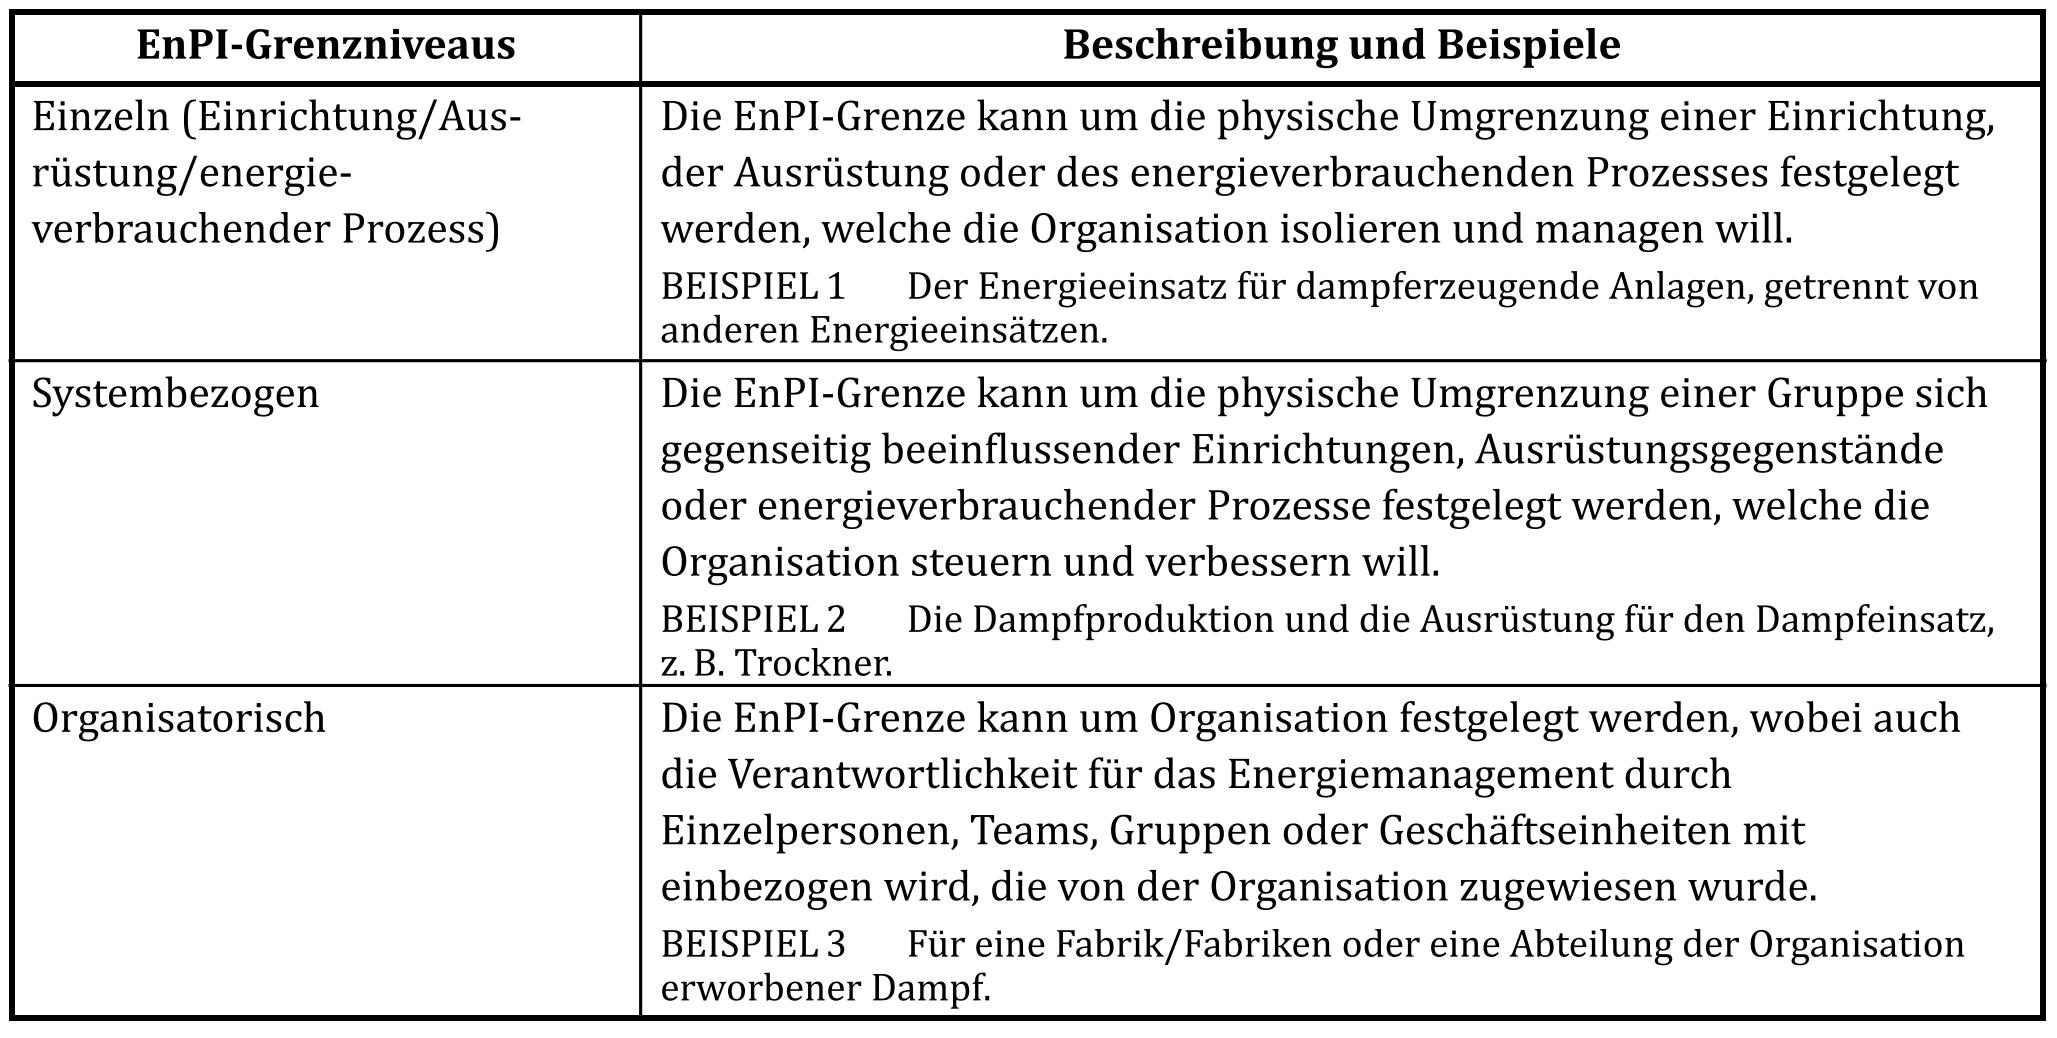
\includegraphics[width=1\textwidth]{../../Ressourcen/Abbildungen/EnPI_Grenzniveaus_ISO_50006.jpg}
    \caption{Die drei EnPI-Grenzniveaus. (Darstellung der E DIN ISO 50006:2024-07 (2024, S. 16))}
    \label{fig:EnPI_Grenzniveaus}
\end{figure}
In Organisationen die keine materiellen Güter Produzieren, also alle Organisationen des tertiären Wirtschaftssektors, eignen sich Gebäude am besten zur 
Abgrenzung der EnPIs (\cite[S. 9]{Fichera.2020}). 
Auf dem ersten Grenzniveau (Einzeln, vgl. Abbildung \eqref{fig:EnPI_Grenzniveaus}) kann eine Energieleistungskennzahl definiert werden, indem der Energieeinsatz 
zur Bereitstellung einer spezifischen Energiedienstleistung durch eine einzelne Anlage erfasst wird. Da die Energiedienstleistung als energieverbrauchender 
Prozess gilt, dient sie als Grundlage zur Eingrenzung der EnPI.
Systembezogen kann folglich eine Energieleistungskennzahl definiert werden, indem der Energieeinsatz zur Bereitstellung einer zusammenhängenden Energiedienstleistung 
unter Berücksichtigung mehrere miteinander verbundene Prozesse oder Anlagen, die gemeinsam zur Erbringung dieser Energiedienstleistung beitragen erfasst werden. 
Organisatorisch können EnPI-Grenzen anhand der organisatorischen Struktur, also zum Beispiel der Einteilung eines Gebäudes in Gebäudezonen und Arbeitsgruppen und -teams 
festgelegt werden.
\subsection{Identifikation wesentlicher Energieeinsätze}

\subsubsection{Analyse und Unterscheidung von Energieeinsätzen}

Die DIN EN ISO 50001:2018-12 verpflichtet Organisationen im Rahmen der Planungsphase des PDCA-Zyklus zur Identifikation von wesentlichen Energieeinsätzen auf Grundlage 
der vorher durchgeführten Datenanalyse (\cite[S. 25]{DIN50001.2018}).
Die Norm definiert einen Energieeinsatz als Anwendung von Energie zum Beispiel für Energiedienstleistungen wie Lüftung oder Heizung, und bezeichnet den Begriff mitunter als 
Endnutzung von Energie (\cite[Kapitel 3.5.4]{DIN50001.2018}). 
Der Energieeinsatz ergibt sich aus dem Produkt des spezifischen Energieeinsatzes und der Menge der Nachgefragten Energiedienstleistungen (vgl. Gleichung \eqref{EnergieeinsatzMiller}) (\cite[S. 120]{Miller.2016}).
Der Spezifische Energieeinsatz ergibt sich aus dem Kehrwert der Energieeffizienz (vgl. Gleichung \eqref{EffizienzgleichungMiller}) (\cite[S. 120]{Miller.2016}).
\begin{equation}
    \text{Energieeinsatz} := \text{Spezifischer Energieeinsatz} \cdot \text{Menge Energiedienstleistung}
    \label{EnergieeinsatzMiller}
\end{equation}

\begin{equation}
    \text{Spezifischer Energieeinsatz} :=\frac{\text{Aufwand}}{\text{Erreichter Nutzen}}
    \label{SepzifischerEnergieinsatzMiller}
\end{equation}

Betrachtet man beispielsweise eine Heizungsanlage als nutzenseitige Energiedienstleistung im Untersuchungsgegenstand Gebäudezone.
So könnte man den erreichten Nutzen mit der Grundfläche konkretisieren. 
Der Aufwand wird durch den im Bilanzzeitraum anfallenden Nutzenergiebedarf zur befriedigung der Energiedienstleistung: Heizung gemessen.
Der Spezifische Energieeinsatz ist somit der im Bilanzzeitraum entstandene Nutzenergiebedarf zum Heizen pro Quadratmeter. 

Ein wesentlicher Energieeinsatz, auch SEU (en: significant energy use), wird von der Norm als Energieeinsatz der wesentlichen Anteil am Energieverbrauch 
hat und/oder erhebliches Potential für eine Verbesserung der energiebezogenen Leistung bietet definiert (\cite[Kapitel 3.5.6]{DIN50001.2018}). 
SEUs können Anlagen beziehungsweise Standorte, Systeme, Prozesse oder eine Einrichtungen sein (\cite[Kapitel 3.5.6]{DIN50001.2018}).
Zur Definition von Kriterien zur Identifikation von SEUs macht die Norm keine Angaben und verpflichtet die Organisation die die Norm anwendet zur Entscheidung was 
als wesentlicher Energieeinsatz anzusehen ist (\cite[S. 38]{DIN50001.2018}). 
Neben Energieerzeugungsanlagen und Umwandlungsanlagen gibt es Anlagenkategorien für Klimatisierungsanlagen, 
Lüftungsanlagen, Bleuchtungsanlagen sowie Informations- und Kommunikationstechnik (\cite[S. 14]{Hohnhold.2013}).

Eine differenzierte Darstellung der Verbrauchsstrukturen nach Anlagenkategorien beziehungsweise einzelner Anlagen ermöglicht das identifizieren von 
wesentlichen Energieeinsätzen und liefert somit auch Ansatzpunkte zur Verbesserung der Energieeffizienz (\cite{Fink.1997} zitiert nach \cite[S. 8]{Hohnhold.2013}).
Die in Abbildung \eqref{fig:Disagggregation_Bilanzraum_Nutzengrößen} dargestellte Disaggregation eines Bilanzraums nach Nutzengrößen kann bei der Analyse der 
Verbrauchsstrukturen innerhalb eines Untersuchungsgegenstands im Rahmen der Datenanalyse beitragen.



Abbildung \eqref{fig:Disagggregation_Bilanzraum_Nutzengrößen_Beispiel} zeigt Beispielhaft wie die Disagggregation von Bilanzräumen zur Identifikation von 
wesentlichen Energieeinsätzen beitragen kann. 
Der durch die aufwandsseitigen Ressourcen gedeckte Nutzenergiebedarf der bilanzierten Energiedienstleistung kann als absolute Energieleistungskennzahl zur 
Bewertung des Energieeinsatzes für die Energiedienstleistung betrachtet werden.
Der Energieeinsatz kann mit der durch die Bewertungseinheit quantifizierten Energiedienstleistung in relation gesetzt werden um den Spezifischen Energieeinsatz 
(vgl. Gleichung \eqref{SepzifischerEnergieinsatzMiller}) zu ermitteln, welcher als Beziehungszahl kategorisiert werden kann und somit geeignet zur Bewertung der Energieeffizienz ist. 
Die Integration einer Gliederungszahl als EnPI welche den Energieeinsatz eines Bilanzraums einer Energiedienstleistungen in Relation 
zum Energieeinsatz eines Bilanzraums aller Energiedienstleistungen setzt kann (vgl. Gleichung \eqref{Anteil_Gesamtenergieverbrauch}) den Vergleich des Anteils einzeln Energiedienstleistungen 
am Gesamtenergieverbrauch unterstützen.


\begin{equation}
    \text{Anteil Gesamtenergieverbrauch} :=\frac{\text{Energieverbrauch Bilanzraum}}{\text{Gesamtenergieverbrauch}}
    \label{Anteil_Gesamtenergieverbrauch}
\end{equation}

In diesem Beispiel macht die Heizungsanlage des Hauptgebäudes mit einem Energieeinsatz von 18.750 kWh 62,5 \% des Gesamtenergieverbrauchs aus und hat somit einen 
wesentlich Größeren Anteil am Gesamtenergieverbrauch als die Kühlungsanlage des Hauptgebäudes, welche mit einem Energieeinsatz von 3.750 kWh nur 12,5 \% des 
Gesamtenergieverbrauchs ausmacht.
Mit \( 125 \,\frac{\text{kWh}}{\text{m}^2} \) hat die Heizung den höchsten spezifischen Energieeinsatz und somit die geringst Energieeffizienz und die Kühlung 
mit \( 25 \,\frac{\text{kWh}}{\text{m}^2} \) den geringsten spezifischen Energieeinsatz und somit die höchste Energieeffizienz.

\begin{figure}[H]
    \centering
    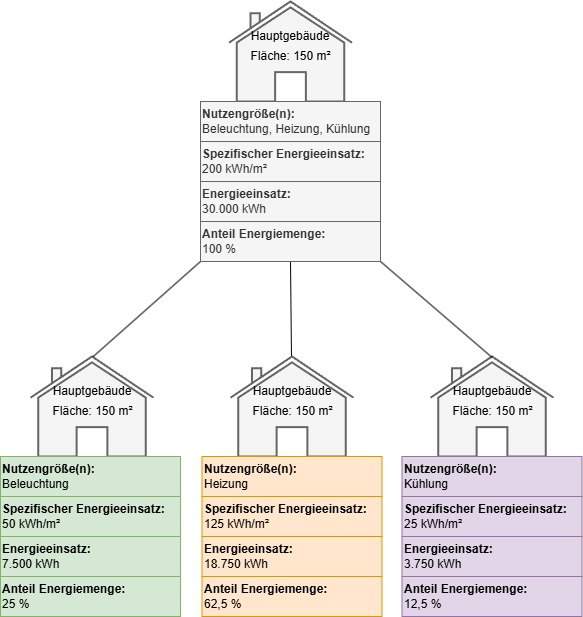
\includegraphics[width=0.7\textwidth]{../../Ressourcen/Abbildungen/Nutzengröße_Bewertungseinheit_Zerlegt_Beispiel.jpg}
    \caption{Beispiel: Disaggregation nach Nutzengrößen. (Eigene Darstellung)}
    \label{fig:Disagggregation_Bilanzraum_Nutzengrößen_Beispiel}
\end{figure}


Eine Analyse der Gebäudezonen innerhalb eines Gebäudes durch Disagggregation nach Untersuchungsgegenstand wie sie in 
\eqref{fig:Disagggregation_Bilanzraum_Untersuchungsgegenstand} visualisiert ist kann zur Identifikation wesentlicher Energieeinsätze durch die Analyse und Unterscheidung 
von Energieeinsätzen innerhalb von Gebäude(-zonen) beitragen.



Abbildung \eqref{fig:Disagggregation_Bilanzraum_Untersuchungsgegenstand_Beispiel} visualisiert beispielhaft, wie eine Disagggregation des Untersuchungsgegenstands 
zur Analyse und Unterscheidung von Energieeinsätzen innerhalb eines Untersuchungsgegenstands beitragen kann.
Zur Bewertung der einzelnen Bilanzräume werden die selben Energieleistungskennzahlen wie in Abbildung \eqref{fig:Disagggregation_Bilanzraum_Nutzengrößen_Beispiel} 
genutzt, allerdings wird der Bilanzraum anhand des Untersuchungsgegenstands disaggregiert.
In diesem Beispiel macht die Gebäudezone 2 mit einem Energieeinsatz von 18.000 kWh 60\% des Gesamtenergieverbrauchs des Gebäudes aus während Gebäudezone 3 mit 
einem Energieeinsatz von 3.000 kWh nur 10\% des Gesamtenergieverbrauchs ausmacht.
Der spezifische Energieeinsatz ist in Gebäudezone 2 mit  \( 300 \,\frac{\text{kWh}}{\text{m}^2} \) am höchsten und somit ist die Energieeffizienz am geringsten. 
In Gebäudezone 3 ist mit \( 100 \,\frac{\text{kWh}}{\text{m}^2} \) der spezifische Energieeinsatz am niedrigsten und die Energieeffizienz somit am höchsten.



\begin{figure}[H]
    \centering
    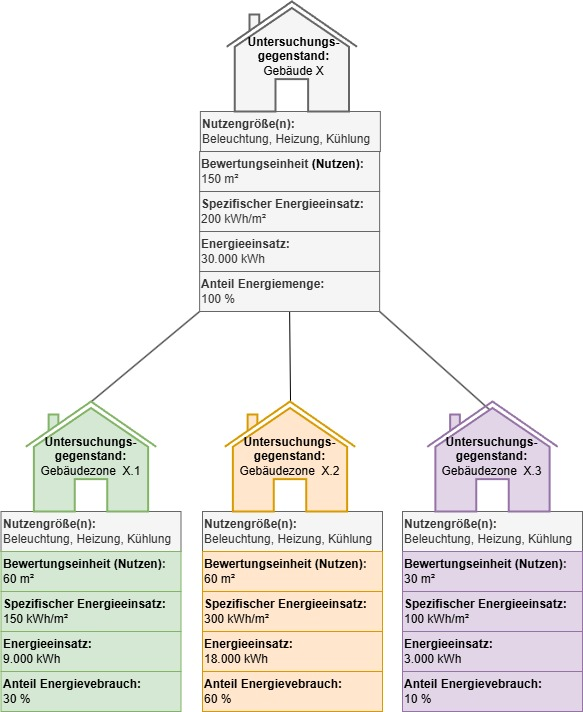
\includegraphics[width=0.7\textwidth]{../../Ressourcen/Abbildungen/Untersuchungsgegenstand_Zerlegt_Beispiel.jpg}
    \caption{Beispiel: Disaggregation nach Untersuchungsgegenstand. (Eigene Darstellung)}
    \label{fig:Disagggregation_Bilanzraum_Untersuchungsgegenstand_Beispiel}
\end{figure}
\subsection{Methodik zur Erfüllung von ISO 50001 Anforderungen}

\subsubsection{Integration von relevanten Variablen}
Relevante Variablen werden von der DIN EN ISO 50001:2018-12 (Kapitel 3.4.9) als quantifizierbarer Faktor, der die energiebezogene Leistung wesentlich beeinflusst sich 
routinemäßig ändert definiert. 
Die relevanten Variablen dürfen gemäß E DIN ISO 50006:2024-07 entweder direkt gemessen oder aus Messungen abgeleitet werden (\cite[S. 18]{DIN50006.2024}).
Beispiele für relevante Variablen sind Wetterbedingungen, Betriebsbedingungen wie Innenraumtemperatur oder Lichtstärke und Arbeitsstunden (\cite[Kapitel 3.4.9]{DIN50001.2018}).
Die Integration von relevanten ist einer der Grundlegenden Anforderungen zur erfüllung von Anforderungen der DIN EN ISO 50001:2018-12.
So sollen im rahmen der Bestimmtung der EnPI-Grenzen Organisationen die für die einzelnen Grenzen relevanten Variablen bestimmen (\cite[S. 17]{DIN50006.2024}).
Für die statistische Analyse der EnPI-Werte ist es notwendig dass der Energieverbrauch und die Daten der zugehörigen relevanten Variablen 
die gleichen Zeitintervalle umfassen (\cite[S. 20]{DIN50006.2024}).
Zur ermittlung wesentlicher Energieeinsätze ist ebenfalls nicht nur die Messung deren Energieverbrauchs notwendig, sondern auch die Messung und Überwachung der 
relevanten Variablen bezüglich SEUs (\cite[S. 23]{DIN50001.2018}). 
Die erfassung dient unter anderem der Bewertung der energiebezogenen Leistung unter gleichwertigen Bedingungen (\cite[S. 8]{DIN50006.2024}). 
Die Auswirkungen der relevanten Variablen werden unter Anwendung des Prozesses der Normalisierung berücksichtigt (\cite[S. 8]{DIN50006.2024}).
Die identifikation relevanter Variablen kann unter der Erwägung von Eingangsgrößen, Prozessen, Ergebnisgrößen und der Umgebung angegangen werden 
(vgl. Abbildung \eqref{fig:Erwägungen_Identifizierung_Rel_Var}).

\begin{figure}[H]
    \centering
    \includegraphics[width=1\textwidth]{../../Ressourcen/Abbildungen/Erwägungen_relevanter_Variablen.jpg}
    \caption{Erwägungen für die Identifizierung von Variablen. (Dargestellt von der E DIN ISO 50006:2024-07 (S. 18))}
    \label{fig:Erwägungen_Identifizierung_Rel_Var}
\end{figure}



\subsubsection{Datengetriebener Ansatz}

Die DIN EN ISO 50001:2018-12 schreibt einen Datengetriebenen Ansatz vor indem Sie von Organisationen welche die Norm umsetzen möchten fordert dass ein Plan zur 
Überwachung und Messung der Hauptmerkmale erstellt und dokumentiert wird (\cite[S. 30ff.]{DIN50001.2018}).
Um die genauen Vorgaben der DIN EN ISO 50001:2018-12 zur ermittlung von Energieeinsätzen zu formulieren, wurde die E DIN ISO 50006:2024-07 veröffentlicht,
welche sich mit der Messung der energiebezogenen Leistung im Rahmen der DIN EN ISO 50001:2018-12 befasst (\cite[S. 1]{DIN50006.2024}).

Organisationen sollen nach E DIN ISO 50006:2024-07 (Kapitel 5.1) Arten des Energieeinsatzes identifizieren und zum einen deren aktuellen, sowie früheren 
Energieverbrauch, zum anderen die aktuelle und frühere Energieeffizienz auf Basis von Messungen und anderen Daten bewerten. 
SEUs werden dann anhand der Analyse dieser Informationen, unter berücksichtigung von Faktoren die die energiebezogene Leistung beeinflussen, 
identifiziert (\cite[Kapitel 5.1]{DIN50006.2024}). 
Die Komplexität der Umsetzung ist dabei nicht vorgeschrieben und kann von einfachen Zählwerten bis hin zu umfangreichen Werten aus Überwachungs- und Messsystemen mit
Softwareanwendung reichen (\cite[S. 36]{DIN50001.2018}).
Folglich bestimmt die Komplexität der Energiedatensammlung auch die potentielle Komplexität der Abbildung und Energiebilanzierung 
des Organisationskontext über Bilanzräume. 
Die Datengetriebenen Ermittlung von Energieeinsätzen in Bilanzräumen fordert folglich die Energiedatensammlung der Energieeinsätze, 
zu der auch die DIN EN ISO 50001:2018-12 Vorgaben macht.

Bei der Auswahl von EnPIs sollen Organisationen ihre vorhandenen Fähigkeiten zur Messung und Überwachung in Bezug auf den 
Energiverbrauch und relevante Variablen berücksichtigen (\cite[S. 21]{DIN50006.2024}).
So muss eine Organisation die Energieflüsse die eine EnPI-Grenze überschreiten messen, wobei die gemessenen Daten sowohl die 
zugelieferte als auch vor Ort erzeugte Energie berücksichtigt die die EnPI-Grenze überschreitet und gespeichert wird (\cite[S. 17]{DIN50006.2024}).
Folglich beeinflusst die Komplexität der Energiedatensammlung die Menge der abbildbaren Energieleistungskennzahlen. 
Eine Organisation soll also die sich auf den Energieverbrauch beziehenden Daten und relevanten Variablen für jede EnPI spezifizieren und erfassen (\cite[S. 18]{DIN50006.2024}).
Falls einige EnPIs aufgrund begrenzter Daten oder anderen Hürden nicht messbar sein, soll die Organisation die EnPIs bewerten und in Folge überarbeiten oder 
zusätzliche Zähler, Messungen oder Modellierungsverfahren einführen (\cite[S. 18]{DIN50006.2024}).

Die DIN EN ISO 50001:2018-12 (2018, Kapitel 6.6, A.6.6) stellt Qualitätskriterien an die Energiedatensammlung in Organisationen.
Die Norm verpflichtet Organisationen dazu, Hauptmerkmale ihrer Tätigkeiten, die sich auf die energiebezogene Leistung auswirken, zu identifizieren und diese in geplanten
Zeitabständen zu messen, zu überwachen und zu analysieren (\cite[S. 23]{DIN50001.2018}).
So muss eine geeignete Abtastzeit der Datensammlung gewählt werden (\cite[S. 20]{DIN50006.2024}), und im Rahmen von Analysen müssen Einschränkungen der Daten 
wie Genauigkeit, Präzision und Konsistenz der Energiedatenerfassung Rechnung getragen werden (\cite[S. 37]{DIN50001.2018}).  
Da sich die DIN EN ISO 50001:2018-12 auf die Veränderung der energiebezogenen Leistung bezieht ist die Wiederholbarkeit ein wichtigeres Qualitätskriterium der 
Energiedatensammlung als die Präzision der Messung (\cite[S. 3]{Szajdzicki.2017}).



%%%%%%%%%%%%%%%%%%%%%%%%%% Konzept %%%%%%%%%%%%%%%%%%%%%%%%%%

\chapter{Konzeption und implementation in EMS-EDM Prophet®}
\section{Anforderungen an das Bilanzraumkonzept}

Dieser Abschnitt befasst sich mit den im Kapitel 2 erarbeiteten Erkenntnissen und formuliert deren Grundlage Anforderungen an das Bilanzraumkonzept.
Zur formulierung der Anforderungen werden Herausforderungen welche sich aus den Grundlagen der Energiebilanzierung und aus den betrachteten Konzepten zur Abbildung 
von Energiebilanzen ergeben betrachtet.
Des weiteren werden Anforderungen auf Grundlage der Angaben der DIN EN ISO 50001:2018-12 zu Energiemanagementsystemen in den Aspekten: 
Energieleistungskennzahlen und wesentliche Energieeinsätze erarbeitet.
Die erarbeiteten Anforderungen sind in Tabelle \eqref{tab:funktionale_anforderungen} dargestellt.


\begin{longtable}{| m{0.06\textwidth} | m{0.16\textwidth} | m{0.38\textwidth} | m{0.4\textwidth} |}
    \caption{Funktionale Anforderungen an das Bilanzraumkonzept auf Basis der theoretischen Erkenntnisse.} \\
    \label{tab:funktionale_anforderungen} \\ 
    
    \hline
    \textbf{Index} & \textbf{Aspekt} & \textbf{Anforderung} & \textbf{Begründung} \\
    \hline
    \multicolumn{4}{|c|}{\textbf{Grundlegende strukturelle Anforderungen an das Datenbankschema}}\\
    \hline
    1 
    & Definition von Energieströmen, -quellen und -senken in Bilanzräumen
    & Im Bilanzraumkonzept \textbf{müssen} für jeden Bilanzraum beliebig viele zu- und abfließende Energieströmen, Energiequellen und Energiesenken definiert werden können. 
    & Die mathematische Beschreibung der Bilanzierung nach Ahrendts (vgl. Gleichung \eqref{BilanzierungsgleichungAhrendt}) beschreibt die Veränderung der bilanzierten 
    Zustandsgröße in abhängigkeit von Zustandsströmen, -quellen und -senken. \\
    \hline
    2
    & Definition des Untersuchungsgegenstands 
    & Im Bilanzraumkonzept \textbf{muss} für jeden Bilanzraum ein Untersuchungsgegenstands definiert werden können. 
    & Der Untersuchungsgegenstand beeinflusst die Systemgrenze einer Bilanz (\cite[S. 109]{Miller.2016}). \\
    \hline
    3
    & Zeitliche Abgrenzung 
    & Das Bilanzraumkonzept \textbf{muss} die Möglichkeit bieten, die Bilanzierung in einem Bilanzraum durch ein Zeitintervall zeitlich abzugrenzen. 
    & Die Zustandsgröße der Bilanz ist nach der Mathematischen Beschreibung von Ahrendts (vgl. Gleichung \eqref{BilanzierungsgleichungAhrendt}) abhängig vom Zeitintervall, 
    in dem Energieströme, -quellen und -senken die Bilanz beeinflussen. \\
    \hline
    4
    & Integration von Energiespeichern 
    & Das Bilanzraumkonzept \textbf{muss} die Abbildung und Integration von energiespeichernden Komponenten ermöglichen. 
    Im zuge der Integration von energiespeichernden Komponenten \textbf{müssen} dem Energiespeicher zu- und abfließende Energieströme 
    abbilden. 
    & Energiespeicher wirken sich nach der Mathematischen Beschreibung einer Energiebilanz nach Rönsch (vgl. Gleichung \eqref{energiebilanzierungsgleichung_Rönsch}) 
    auf das Verhalten der bilanzierten Zustandsgröße aus.
    Energiespeicher nehmen Energie auf und geben sie zeitversetzt ab (\cite[S. 1]{Rathgeber.2018}). \\
    \hline
    5
    & Bewertungs-einheiten eines Bilanzraums 
    & Das Bilanzraumkonzept \textbf{muss} alle Energieströme, -quellen und -senken in der Einheit kWh und derem vielfachen unabhängig von Energieformen und Energieträger 
    in einem Bilanzraum abbilden können. 
    & Die bevorzugte Bewertungseinheit für Energieformen ist kWh und deren Vielfaches (\cite[S. 65]{Konstantin.2023}).\\
    \hline
    6
    & Quantifizierung von Energiedienstleistungen & 
    Das Bilanzraumkonzept \textbf{muss} in Anlehnung an das von Miller (2016) entworfene Konzept der Bewertungsräume aus einem Bilanzraum austretende Energieströme 
    in Form von Energiedienstleistungen mit einer Bewertungseinheit konkretisieren und quantifizieren können. 
    & Das in der Energiewertschöpfungskette (vgl. Abbildung \eqref{fig:Energieflussschema_Posch}) visualisierte Problem:
    dass Energie in unterschiedlichen Formen auftritt und insbesondere im Rahmen der Bilanzierung von Gebäudeenergie zufließende Energieströme in Form von messbarer 
    Endenergie auftreten während die abfließenden Energieströme in Form nicht messbarer Energiedienstleistungen auftreten können wird durch die von 
    Miller (2016) beschriebene Quantifizierung von Energie in Form von Energiedienstleistungen adressiert. \\
    \hline
    7
    & Disaggregation von Bilanzräumen
    & Das Bilanzraumkonzept \textbf{muss} die Disaggregation von Bilanzräumen in Teilbilanzräume abbilden können. 
    & Nach Engelmann (2015) und Miller (2016) haben Bilanzräume die Eigenschaft der Zerlegbarkeit.\\
    \hline
    8
    & Aggregation zufließender Energieströme 
    & Das Bilanzraumkonzept \textbf{soll} in Anlehnung an das von Miller (2016) entworfene Konzept der Bewertungsräume eine Aggregation mehrerer zufließender 
    Energieströme zu einem zufließenden Energiestrom in Bilanzräumen abbilden können. 
    & Mehrere einfließende Energieströme und Energiequellen können zur Deckung des Nutzenergiebedarfs der gleichen Energiedienstleistung beitragen,
    weshalb ihre Aggregation notwendig ist um Rückschlüsse auf den Energieverbrauch einer Energiedienstleistung zu ziehen. \\
    \hline
    9
    & Definierbarkeit der Bilanzraumgrenzen nach Grenzniveaus der E DIN ISO 50006:2024-07 
    & Ein Bilanzraum im Bilanzraumkonzept \textbf{muss} nach allen von der E DIN ISO 50006:2024-07 definierten EnPI-Grenzniveaus (vgl. Abbildung \eqref{fig:EnPI_Grenzniveaus}) abgegrenzt werden können. 
    & Die räumliche und zeitliche Abgrenzung eines Bilanzraums beeinflusst die Berechnung und Vergleichbarkeit von EnPI-Werten (\cite[S. 6]{Hohnhold.2013}). \\
    \hline
    \multicolumn{4}{|c|}{\textbf{Strukturelle Anforderungen an das Datenbankschema}}\\
    \multicolumn{4}{|c|}{\textbf{zur Unterstützung bei DIN EN ISO 50001:2018-12 Anforderungen }}\\
    \hline
    10
    & Definierbarkeit von Energieleistungskennzahlen 
    & Das Bilanzraumkonzept \textbf{muss} die Definition von Energieleistungskennzahlen (EnPIs) in einem Bilanzraum ermöglichen. 
    & Energieleistungskennzahlen sind zentral für die Bewertung der energiebezogenen Leistung im Energiemanagement nach ISO 50001. \\
    \hline
    11
    & Definierbare Arten von Energieleistungskennzahlen
    & Das Bilanzraumkonzept \textbf{muss} in einem Bilanzraum EnPIs der Art: absolute Zahlen sowie Index-, Beziehungs- und Gliederungszahlen definieren können. &
    Unterschiedliche Arten von Kennzahlen bieten unterschiedliche Perspektiven auf die Bewertung eines Bilanzraums. \\
    \hline
    12
    & Integration der energetischen Ausgangsbasis 
    & Das Bilanzraumkonzept \textbf{muss} in einem Bilanzraum für alle definierten EnPI eine energetische Ausgangsbasis bereitstellen und im Bezugszeitraum aggregieren können.  
    & Die Differenz zwischen der Ausgangsbasis und dem EnPI-Wert bestimmt die Verbesserung der Energieeffizienz (vgl. Abbildung \eqref{fig:Beziehung_EnPI_EnB_ISO_50006}).
    Da die Berechnung einer EnB mit einem anhand eines Energiemodells berechnet wird ist die Berechnung der EnBs kein Aspekt dieser Anforderung \\
    \hline
    13
    & Definition von operativen Energiezielen 
    & Das Bilanzraumkonzept \textbf{muss} die Möglichkeit bieten, für einen definierten EnPI ein operatives Energieziel anzugeben und dessen Erfüllung zu evaluieren. 
    & Die Bewertung der Zielerreichung ist essenziell für die kontinuierliche Verbesserung der energiebezogenen Leistung (vgl. Abbildung \eqref{fig:Beziehung_EnPI_EnB_ISO_50006}). \\
    \hline
    14
    & Integration von relevanten Variablen
    & Das Bilanzraumkonzept \textbf{muss} für jeden Bilanzraum die Möglichkeit bieten, relevante Variablen zu definieren. 
    & Die Integration von relevanten Variablen ist einer der Grundlegenden Anforderungen zur erfüllung von Anforderungen der DIN EN ISO 50001:2018-12.
    Sie müssen unter anderem im Rahmen der Definition von EnPI-Grenzen bestimmt werden (\cite[S. 17]{DIN50006.2024})  \\
    \hline
    \multicolumn{4}{|c|}{\textbf{Anforderungen an die Datenauswertung der Bilanzräume}}\\
    \multicolumn{4}{|c|}{\textbf{zur Unterstützung bei DIN EN ISO 50001:2018-12 Anforderungen }}\\
    \hline
    15
    & Zeit-Werte-Verlauf von EnPI und EnB 
    & Das Bilanzraumkonzept \textbf{muss} den Zeit-Werte-Verlauf für alle im Bilanzraum definierten EnPIs und die dazugehörige EnBs ausgeben können. 
    & Eine zeitabhängige Analyse ermöglicht Erkenntnisse über das zeitabhängige Verhalten und den Einfluss relevanter Variablen (\cite[S. 14]{DIN50006.2024}). \\
    \hline
    16
    & Abbildbare Kennzahlenarten 
    & Das Bilanzraumkonzept \textbf{muss} in einem Bilanzraum EnPIs der Art: absolute Zahlen sowie Index-, Beziehungs- und Gliederungszahlen berechnen können. &
    Unterschiedliche Arten von Kennzahlen bieten unterschiedliche Perspektiven auf die Bewertung eines Bilanzraums. \\
    \hline
    17
    & Zeitlichen Aggregation von EnPI-Werten 
    & Für jeden in einem Bilanzraum definierten EnPI \textbf{müssen} die dazugehörigen EnPI-Werten zu einem EnPI-Wert über das im Bilanzraum definierte Zeitintervall aggregieren können. 
    & Die zeitliche Aggregation erlaubt eine Bewertung der energiebezogenen Leistung über einen Berichtszeitraum hinweg und ermöglicht den Vergleich mit dem EnB zur ermittlung der Energiebezogenen Leistung 
    (vgl. Abbildung \eqref{fig:Beziehung_EnPI_EnB_ISO_50006}). \\
    \hline
    18
    & Bestimmung des Energieeinsatzes
    & Für jeden Bilanzraum im Bilanzraumkonzept \textbf{muss} der Energieeinsatz in einem Bilanzzeitraum berechnet werden können. 
    & Auf Grundlage des Vergleichs von Energieeinsätzen können nach DIN EN ISO 50001:2018-12 wesentliche Energieeinsätze auf Grundlage 
    der von der Organisation festgelegten Kriterien identifiziert werden. \\
    \hline
    19
    & Bestimmung des spezifischen Energieeinsatzes
    & Für jeden Bilanzraum im Bilanzraumkonzept der den Energievebrauch einer Energiedienstleistungen bilanziert \textbf{muss} der spezifische Energieeinsatz 
    (vgl. Gleichung \eqref{SepzifischerEnergieinsatzMiller}) in einem Bilanzzeitraum berechnet werden können. 
    & Der spezifische Energieeinsatz kann als Maß der Energieeffizienz bei der Erfüllung einer Energiedienstleistung genutzt werden und somit Bilanzräume mit Potential zur 
    Energieeinsparung aufzeigen. \\
    \hline
    20
    & Auswertung von Energieeinsätzen in Disaggregierten (Teil-)Bilanzrräumen
    & Das Bilanzraumkonzept \textbf{muss} Funktionen zur Analyse des Energieeinsatzes eines Bilanzraums im Verhältnis zu seinen disaggregierten Teilbilanzräumen bereitstellen.
    & Die Analyse des Energieeinsatzes in Teilbilanzräumen im Verhältnis zum Gesamtbilanzraum ermöglicht die Erfassung des Anteils des Energieverbrauchs des 
    Teilbilanzraums am Gesamtenergieverbrauch \\
    \hline 
\end{longtable}
Quelle: Eigene Darstellung basierend auf den Erkenntnisse aus Kaptiel 2: Stand der Forschung und Theoretische Grundlagen.

\section{Ist-Zustand des Datenbankschemas von EMS-EDM Prophet®}

Im Folgenden wird der aktuelle Zustand des für den Problemraum relevanten Segments des Datenbankschemas des Energiemanagementsystems EDM-EMS-Prophet® in der Version 14.1 erläutert.
Das System basiert auf der \textit{Oracle Database 19c Standard Edition 2} (Release 19.0.0.0.0 – Production). 
Die Struktur des Datenbankschemas ist in Abbildung \eqref{fig:Datenbankschema_Prophet_ZRM} dargestellt.

\subsubsection{Zeitreihenmanagement}
Im Zentrum des betrachteten Segment des Datenbankschemas steht die Tabelle: ZRM\_ZR. 
Sie dient als zentrale Tabelle zur Verwaltung der im Energiemanagementsystem gespeicherten Zeitreihen und weist jeder Zeitreihe eine eindeutige ID zu.
Neben der ID enthält die Tabelle die Bezeichnung einer Zeitreihe, den Typ einer Zeitreihe  welcher zwischen M-Messwert, P-Prognose 
und F-Fahrplan variieren kann und einigen weiteren Spalten.

Die Tabelle steht in N:1 Beziehung zur Tabelle ZRM\_AZ welche Informationen bezüglich Abtastzeiten von Zeitreihen speichert. 
In ZRM\_AZ wird unter anderem die ID, Zeitzone, die Bezeichnung, der Gültigkeitszeitraum, das Zeitintervall aufgelöst bis zur Sekunde und das 
Offset aufgelöst bis zu Minute einer Abtastzeit gespeichert.

Des weiteren steht die Tabelle ZRM\_ZR in N:1 Relation zur Tabelle: ZRM\_ME welche Informationen bezüglich Maßeinheiten von Zeitreihen speichert.
In der Tabelle sind neben der ID der Maßeinheit auch deren konkrete Einheit, die Bezeichnung der Größe und weitere Informationen Spalten. 
Eine wichtige Rolle haben die Spalten: ME\_ISBASISEINHEIT welche angibt ob die Maßeinheit eine Basiseinheit darstellt, und wenn dies nicht gilt 
ME\_UFAKTOR welche den Umrechnungsfaktor zur entsprechenden Basiseinheit hält.

Über die N:M Relation zwischen ZRM\_ZR und ZRM\_ZRINFO über ZRM\_ZR\_ZRINFO wird eine Zuweisung von in ZRM\_ZRINFO angelegten Infofeldern 
mit einem in ZRM\_ZR\_ZRINFO vergebenen Wert zu einer Zeitreihe realisiert. 
Die hier abgebildeten Infofelder können als Key-Value Paare für Zeitreihen betrachtet werden, wobei ZRM\_ZRINFO.ZRINFO\_BEZ den Key und 
ZRM\_ZR\_ZRINFO.ZR\_INFO\_TEXT den Wert realisiert.

Über die N:1 Beziehung zwischen ZRM\_ZR und DAT\_MANDANT werden alle Zeitreihen mit einem Mandanten Verknüpft. 
Mandanten können ganze Organisationen oder Teile von Organisationenen repräsentieren und dienen der Zuweisung von Zuständigen für die Zeitreihen. 
So wie die anderen Tabellen enthält diese Tabelle Spalten zur Überwachung von Änderungen und dem Anlegen.

\subsubsection{Zeitreihenwerte}

Die Zeitreihenwerte einer in EDM-EMS-Prophet® gespeicherten Zeitreihe werden in der ZRM\_ZW1 gespeichert, welche in einer N:1 Beziehung zur Tabelle ZRM\_ZR steht.
In der Tabelle werden nur äquidistante Werte, also Werte welche im gleichen Zeitintervall abgetastet werden, abgelegt.
Die drei zentralen Spalten der Tabelle sind ZRM\_ZRID welche die relation zur Zeitreihe realisiert, ZW1\_UT welche den Endzeitstempel eines Werts in UTC hält 
und ZW1\_Wert welche den Zeitreihenwert in der Basiseinheit hält.
Hat man Beispielsweise eine Zeitreihe welche die Messwerte des Energievebrauchs einer Anlage in kWh speichert entspricht der Wert in ZW1\_Wert zum Endzeitstempel 
ZW1\_UT der Energiemenge die in dieser Anlage seit vom vorherhigen Endzeitstempel verbraucht wurde. 
Die Werte in ZRM\_ZW1 stellen somit im Falle von Zeitreihen die die Messergebnisse von Energieströme speichern, Aggregate des Energiestroms über den in ZRM\_AZ 
festgelegten Abtastzeitraum dar.
ZW1\_Version und ZW1\_UPDATE dienen der Versionierung der Werte, da die Zeitreihenwerte angepasst werden können.
Somit ist die Grundlegende Funktionalität Energieströme zu erfassen und zu speichern gegeben. 
Um Bilanzräume abzubilden fehlen folglich Tabellen welche erfasste Zeitreihen in ein durch das Bilanzraumkonzept erarbeite Zusammenhänge bringen und Berechnungnen 
über diese Zeitreihen durchführen.

% \section{Ausgangszustand: EMS-EDM Prophet®}

% \section{Anforderungen}
% \subsection{Modellierung von Bilanzräumen}

% \subsection{Abbildung von Metriken zur Bewertung von Bilanzräumen}

% \subsection{Technische Anforderungen und Datenkommunikation}


% \section{Umsetzungskonzept für EMS-EDM Prophet®}

% \subsection{Systemarchitektur}
% \subsection{Datenmodell und Datenbankdesign}
% \subsection{Technische Umsetzung und Datenkommunikation}
% \subsection{EnPI Abbildung}
% \subsection{Test- und Validierungskonzept}
% \subsection{Sicherheitskonzept}
% \subsection{Bedingungen und Anforderungen an die Laufzeitumgebung}

% \section{Technische Realisierung}
% In diesem Kapitel sollen alle technischen Aspekte der Umsetzung beschrieben werden.
% \section{Umsetzungsablauf}
% In diesem Kapitel soll der Ablauf der Umsetzung beschrieben und begründet werden.
% \section{Ergebnis}
% In diesem Kapitel soll das Ergebnis der Umsetzung beschrieben werden.
% \subsection{Anforderungsumsetzung}
% In diesem Kapitel soll beschrieben werden wie die Anforderungen umgesetzt wurden und welche Anforderungen umgesetzt wurden.
% \subsection{Vergleich zum bestehenden System}
% In diesem Kapitel soll der Vergleich zum bestehenden System gezogen werden und erläutert werden was sich verändert hat.


%%%%%%%%%%%%%%%%%%%%%%%%%% Implementation und Evaluation %%%%%%%%%%%%%%%%%%%%%%%%%%

\chapter{Evaluation}

% \section{Einleitung}
% \subsection{Ziel der Evaluation}
% \subsection{Methodik}

% \section{Metriken und Kennzahlen}
% \subsection{Definition der Erfolgsmessung}
% \subsection{Quantitative Metriken}
% \subsection{Qualitative Metriken}

% \section{Experimenteller Aufbau}
% \subsection{Beschreibung des Experimentes}
% \subsection{Testumgebung und -bedingungen}
% \subsection{Datensätze und Szenarien}

% \section{Durchführung und Ergebnisse}
% \subsection{Durchführung}
% \subsection{Quantitative Ergebnisse}
% \subsection{Qualitative Ergebnisse}

% \section{Vergleich mit alternativen Ansätzen}

% \section{Diskussion der Ergebnisse}

% \section{Zusammenfassung der Evaluation}

\chapter{Fazit}
% \section{Zusammenfassung der Ergebnisse}
% \section{Ausblick auf zukünftige Arbeiten}

\printbibliography[title={Literaturverzeichnis}]

\appendix
\chapter{Anhang}
\begin{sidewaysfigure}
    \centering
    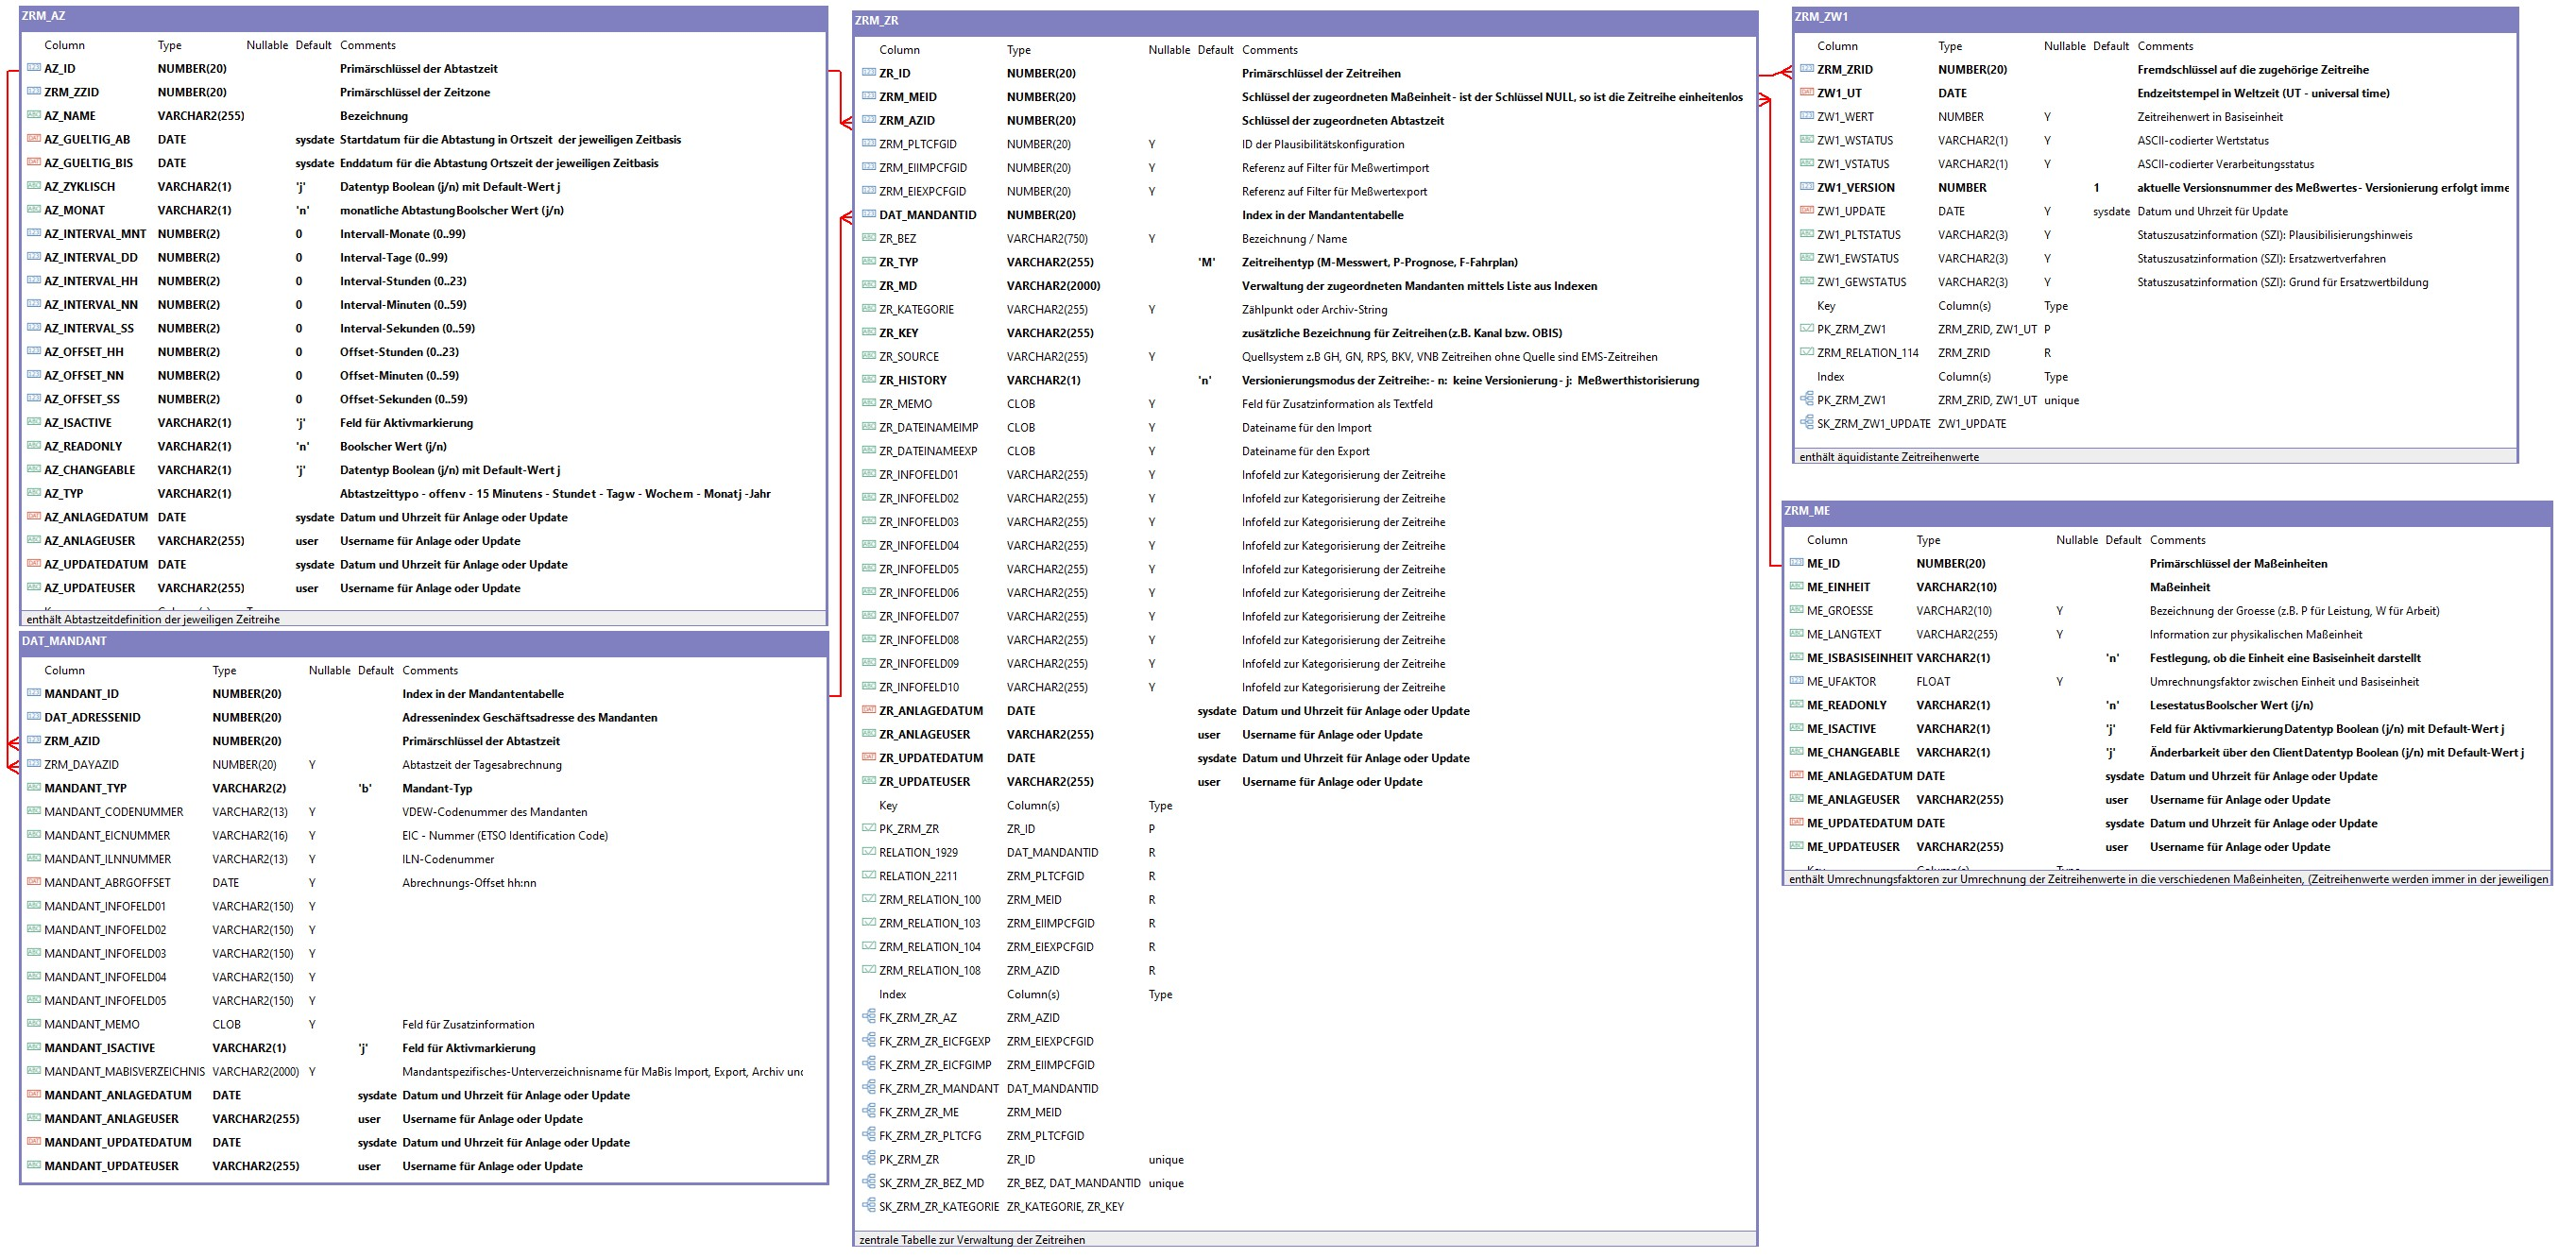
\includegraphics[width=\textwidth]{../../Ressourcen/Abbildungen/Schema_ZRM_ZR.jpg}
    \caption{Teil des Datenbankschemas von EMS-EDM Prophet (Eigene Darstellung)}
    \label{fig:Datenbankschema_Prophet_ZRM}
\end{sidewaysfigure}


\section*{Selbstständigkeitserklärung}

\end{document}
